\documentclass[12pt,spanish, singlespacing,]{MastersDoctoralThesis}
\usepackage[utf8]{inputenc} 
\usepackage[T1]{fontenc} 
\usepackage[none]{hyphenat}
\usepackage{palatino} 
\usepackage{acronym}
\usepackage{amsmath}
\usepackage{float}
\usepackage{multicol}
\usepackage[caption = false]{subfig}
\spacing{1.5}
\usepackage[acronym,nomain]{glossaries}
%\usepackage[backend=bibtex,style=authoryear,natbib=true]{biblatex}
%\addbibresource{main.bib}
\usepackage[autostyle=true]{csquotes}
\usepackage{tikz}
\usetikzlibrary{shapes.geometric, arrows}
\usepackage{smartdiagram}
\usepackage{afterpage}
\tikzstyle{startstop} = [rectangle, rounded corners, minimum width=4cm, minimum height=1.5cm,text centered, draw=black, fill=blue!30]
\tikzstyle{arrow} = [thick,->,>=stealth]
\newcommand\blankpage{%
    \null
    \thispagestyle{empty}%
    \addtocounter{page}{0}%
    \newpage}
    
\usepackage{listings}
\renewcommand{\lstlistingname}{Código}
\renewcommand\lstlistlistingname{Índice de Código}

\usepackage{float}
\usepackage{url}
\makeatletter
\g@addto@macro{\UrlBreaks}{\UrlOrds}
\makeatother

\thesistitle{}
\supervisor{} 
\examiner{} 
\degree{} 
\author{} 
\subject{}
\keywords{} 
\university{\href{http://www.uni.edu.pe/}{Universidad Nacional de Ingenier\'ia}} 
\department{\href{http://fc.uni.edu.pe/fc/index.php/escuelas/ciencia-de-la-computacion}{}} 
\faculty{\href{http://fc.uni.edu.pe/fc/}{}}
\hypersetup{pdftitle=\ttitle} 
\hypersetup{pdfauthor=\authorname}
\hypersetup{pdfkeywords=\keywordnames} 
\sloppy
\decimalpoint
\begin{document}
\frontmatter 
\pagestyle{plain} 
\begin{titlepage}
\begin{center}
%\textsc{\huge \univname}\\[0.5cm]

\begin{figure}[h]
\centering

\includegraphics[width=0.3\textwidth]{Figures/log_uni.png}
\end{figure}

\textsc{\huge \univname}\\[0.3cm]
\textsc{\Large Facultad de Ciencias}\\[0.2cm]
\textsc{\large Escuela Profesional de Ciencia de la Computaci\'on}\\[2cm]
\textsc{\LARGE \textit{Conversión de voz en texto usando redes neuronales}}\\[2cm] 
{\Large \textbf{SEMINARIO DE TESIS 2}}
{\huge \bfseries \ttitle}\\[2cm] 
% Thesis title
%\bigskip
%\HRule \\[0.8cm] % Horizontal line

%\begin{minipage}{1.5\textwidth}
%\begin{flushleft} \large
\bigskip
\bigskip
\large\emph{Autor: Víctor Jesús Sotelo Chico}
{\authorname}\\ 
\large\emph{Asesor: Antonio Morán Cardenas}
{\supname} 
%\end{flushleft}
%\end{minipage}
%\\[2cm]
\\[1cm]
{\large Diciembre, 2018}\\[4cm] 
 
\vfill
\end{center}
\end{titlepage}
\afterpage{\blankpage}
%\cleardoublepage
%\renewcommand{\abstractname}{Abstract}
\begin{abstract}
\addchaptertocentry{\abstractname}
En las últimas décadas el campo de la inteligencia artificial se ha desarrollado rápidamente. Estudios sobre reconocimiento de imágenes y voz han sido estudiados en las últimas décadas. Actualmente este campo requiere realizar un gran números de cálculos para entrenar redes neuronales que sean capaces de distinguir y clasificar distintos objetos contenidos en imágenes. Incluso este proceso puede tardar más dependiendo del tamaño del dataset. Por lo cual surge la necesidad de encontrar métodos que permitan acelerar el proceso de entrenamiento de las redes neuronales.\\
Por tal motivo presente seminario buscar lograr un mayor entendimiento de métodos para acelerar el proceso de entrenamiento de una red neuronal convolucional, basándonos en la teoría de redes neuronales y usando como herramienta la librería tensorflow, esta nos permite un uso controlado de las métodos de optimización.

\textbf{KEYWORDS}:  Dataset, Métodos Adaptativos, CNN, SGD, Optimizadores.
\end{abstract}\hspace{10pt}

\keywords{agasga}


\afterpage{\blankpage}
\tableofcontents
%\afterpage{\blankpage}
\listoffigures
%\afterpage{\blankpage}
%\listoftables
%\afterpage{\blankpage}
%\listoftables 
%\lstlistoflistings
%\afterpage{\blankpage}
\newpage

\begin{center}
{\huge Índice de Acrónimos}\\[2cm]
\end{center}
\bigskip
\begin{tabular}{ l c l }
\textbf{k-nn}& & k- nearest neighbors\\
\textbf{SVM}& & Super Vector Machine\\
\textbf{SVC}& & Super Vector Regression\\
\textbf{SVR}& & Super Vector Classification\\
\textbf{SGD} & & Stochastic gradient descent\\
\textbf{DNN} & & Deep Neural Network\\
\textbf{CNN} & & Convolutional Neural Network\\
\textbf{ETC} & & Etcétera \\

\end{tabular}
\afterpage{\blankpage}

\newpage
\begin{center}
{\huge \textit{Agradecimientos}}\\[1.5cm]
\end{center}

Agradezco a mis padres por todo el apoyo incondicional durante todos estos años de estudio, a mis compañeros de clase por el apoyo brindado durante el tiempo de estudio y a mi asesor por ayudarme en este seminario.



\afterpage{\blankpage}

\mainmatter 
\pagestyle{thesis}
\chapter{Introducción}
%-- 10 lineas
Dentro de la inteligencia artificial, las redes neuronales profundas desempeñan un papel muy importante, debido a que estas permiten entrenar a las computadoras para que realicen tareas que nuestros cerebros realizan de manera natural como el reconocimiento de voz, imágenes y patrones. Una características de las redes neuronales profundas es la gran cantidad de capas que poseen. Esto permite que las redes sean capaces de extraer características de los datos ya sean imágenes o voz. La comunicación entre los seres humanos se realiza por medio del habla, la cual es emitida como una señal de voz debido a la cantidad de información que esta señal posee ha permitido el estudio y desarrollo de aplicaciones como identificadores biométricos, procesamiento de lenguaje natural, etc. Tareas como estas requieren un análisis complejo debido a que se necesita tratar problemas como la reverberación y el ruido presentes en el entorno.




\section{Motivación}
La inteligencia artificial constituye una base muy importante en el campo de la computación, mezcla un conjunto de disciplinas como la estadística y ciencia de la computación con el objetivo de construir modelos que puedan permitir a las computadoras realizar tareas que hace algunos años hubiesen sido considerada imposibles.\\
Actualmente las computadoras son capaces de reconocer objetos y clasificarlo. Esto ha permitido que la industria de la robótica se desarrolle de manera acelerada en las últimas décadas.
 Además hoy en día existen muchas herramientas que nos permiten desarrollar este tema y profundizarlo, pero a medida que aumenta la complejidad del problema, el costo computacional se incrementa, lo cual se convierte en un problema importante.

 Una de la soluciones que surgió fue el uso de la GPU's para acelerar procesos como el entrenamiento de una red neuronal con muchas capas ocultas, las GPU's representan una solución muy eficaz debido a que en el campo de la inteligencia artificial existen muchas tareas que son paralelizables.

Actualmente el mercado de GPU's evoluciona muy rápido debido a su gran demanda en la industria de los videojuegos, este mercado se encuentra dominado por NVIDIA y AMD, esta competencia y la alta demanda permite que las GPU's tengan mejor rendimiento lo cual puede ser usado para obtener mejores resultados en el campo del Aprendizaje Automático. 

Por otro lado, la optimización no solo se basa en el uso de hardwares más potentes, sino también depende de la elección de métodos adecuados para nuestros modelos, esta elección dependerá mucho del problema a tratar. Uno de los métodos más usado en el campo del Aprendizaje Automático es la gradiente de descenso estocástica pero este métodos por sí solo no es muy óptimo. 

Actualmente existe la problemática de hallar métodos más eficientes de optimización que obtengan un mejor rendimiento, el presente seminario se centra en la búsqueda y comparación de estos métodos con el fin de encontrar aquellos que sean más rápidos y eficientes. Además, adquirir el conocimiento y entender cómo es que estos funcionan.
%-----
%-----Que es lo que te ha motivado para realizar la tesis en esta temática y los aspectos más esenciales que pensabas obtener de ella...

%-----Este punto podrá ser de 4 páginas máximo. Es una de las partes más importantes que introduce al lector en el trabajo en tu tesis, por lo que debe estar muy bien redactado y estructurado.

\section{Objetivos}

El objetivo de este seminario es el de mostrar las ventajas del uso de distintos métodos de optimización para acelerar el entrenamiento de una red neuronal convolucional en una tarea de clasificación.

Específicamente, los objetivos de este trabajo con respecto al sistema son:

\begin{itemize}
\item[•] Entender el funcionamiento de las redes neuronales profundas.%--OBJETIVO ESPECÍFICO 1.

\item[•] Estudiar métodos de optimización en Aprendizaje Automático.

\item[•] Conocer las ventajas y desventajas de diferentes métodos de optimización.
\item[•] Mostrar los resultados de distintos métodos de optimización en el entrenamiento de una red neuronal convolucional para tareas de clasificación.



\end{itemize}

Y los objetivos con respecto a las competencias académicas desplegadas en el trabajo son:
\begin{itemize}
\item[•] Desarrollar un mejor entendimiento de las redes neuronales y sus aplicaciones, para así poder lograr afrontar problemas en el campo de la inteligencia artificial. %--OBJETIVO COMPETENCIA 1.
\item[•] Obtener la capacidad de discriminar entre los distintos métodos de optimización y elegir el adecuado para un problema de aprendizaje profundo.%--OBJETIVO COMPETENCIA 2.
\item[•] Obtener un conocimiento de las herramientas y recursos que existen actualmente para abordar problemas de aprendizaje profundo, además de poder analizar que herramientas son adecuadas para algunos problemas.
\end{itemize}

\section{Estructura del Seminario}


\begin{itemize}

\item \textbf{Introducción:} \\
En este capítulo introductorio se comenta sobre el tema a tratar, las motivaciones, intereses, objetivos con los cuales se planteo el presente seminario.
%--En este capítulo introductorio se comenta sobre las motivaciones ...

\item \textbf{Estado del Arte:} \\
Este capítulo muestra los trabajos e investigaciones ya realizadas, además de algunas aplicaciones que motivaron al presente seminario y además las investigaciones mostrarán el interés del problema planteado.

\item \textbf{Aprendizaje automático y Redes Neuronales:} \\
En este capítulo daremos una introducción general al Aprendizaje automático y distinguiremos los tipos de aprendizajes que existen, Además veremos los tipos de problema en esta área. Luego trataremos el tema de las Redes neuronales como una introducción al capítulo 4.
\item \textbf{Optimizadores para la gradiente de descenso en una Red Neuronal Convolucional:} \\
En este capítulo conoceremos más de un tipo específico de redes neuronal, las redes neuronales convolucionales. Detallares las principales diferencias con las redes tradicionales y describiremos sus principales hiperparámetros. Luego de eso nos enfocaremos en los optimizadores de la gradiente de descenso.
\item \textbf{Resultados:} \\
Se mostrarán los resultados obtenidos en las pruebas de los optimizadores además de describir los resultados.
\item \textbf{Conclusiones y Trabajo Futuro:} \\
En este capítulo se plantean las conclusiones y se detalla algunos inconvenientes encontrados durante el trabajo. Además que se comprueba la teoría descrita en el capítulo 4.
%--\item \textbf{Metodología y Herramientas:} \\
%--....

%--\item \textbf{...} \\
%--Un pequeño texto más de ese capítulo(s) en concreto.

%--\item \textbf{Conclusiones y Trabajo a Futuro:}\\
%--En este capítulo se exponen las conclusiones obtenididas de este trabajo. Adicionalmente, se proponen trabajos a futuro para la implementación de el servidor y la aplicación web del sistema.
\end{itemize}

%--NOTA: RECUERDE QUE ES COMO UN LIBRO TODO CAPÍTULO NUEVO COMENZARÁ CON PÁGINA IMPAR NUNCA PAR



%\newpage
%$\ $
%\thispagestyle{empty} % para que no se numere esta pagina
\chapter{Estado del Arte}
En este capítulo se describirán las investigaciones anteriores con relación al Aprendizaje Automático, además de sus aplicaciones. También se verán algunas investigaciones referente al reconocimiento de voz y los algoritmos usados para estas tareas.

Este trabajo también presentará investigaciones referentes a Aprendizaje Profundo, exclusivamente nos enfocaremos a la Redes Neuronales Convolucionales(CNN), ya que son parte del tema de estudio en la presente investigación.

%---Escribir un texto de un o dos párrafo(s) máximo de 10 líneas con una introducción al capítulo 

%---El capítulo estado del arte es tanto o más importante que la tesis en sí. En el se debe especificar que desarrollo relacionado a tu tesis existe ya a nivel global y en que se diferencia tu trabajo de ellos. Por lo tanto un análisis exhaustivo de la especialidad y de los trabajos previos es tanto o más importante que el trabajo en sí, ya que indica un alto conocimiento de la materia si está bien estudiado.

%---En este capítulo van a ir muchas citas \cite{Wan09} de trabajos pero sobre todo de artículos científico, haga un buen estudio del arte \cite{Shuo10,Feldmann03}


\section{GPU computing}
Actualmente, el uso de GPU's permitió lograr aplicaciones que antes se podrían creer imposibles debido a su largo tiempo de ejecución. Hoy en día las GPUs son altamente usadas ya que cuentan con cientos de núcleos de procesadores en paralelo que permiten resolver rápidamente los problemas que son altamente paralelizables.
\subsection{The GPU computing Era}
	El artículo se enfoca principalmente en describir la evolución que sufrieron las arquitecturas de GPUs, además de mostrar la importancia del uso de las GPUs para un mayor rendimiento y eficiencia que antes hubiesen sido consideradas imposibles debido al alto tiempo de ejecución que requerían. Además nos muestra que la escalabilidad es la principal característica que ha permito que las GPUs aumenten su paralelismo y rendimiento.
\section{Aprendizaje Automático}
El uso del Aprendizaje Automático representa una gran ventaja para empresas que manejan gran cantidad de datos debido a que permiten descubrir patrones y analizar los datos.

\subsection{Uso de redes neuronales para encontrar el rendimiento de una GPU}
Un equipo conformado por investigadores \cite{GPU}de AMD y The University of Texas at Austin, fueron quienes propusieron el uso de redes neuronales para predecir el rendimiento de una GPU.
En la actualidad existen empresas dedicadas a la creación de GPUs, en el proceso una parte fundamental es la verificación del rendimiento de las GPUs. Actualmente existen simuladores conocidos como GPGPU-SIM que permiten realizar estimaciones precisas pero estos presentan algunas dificultades como el tiempo empleado en configurarlos en base al hardware real, no obstante, este proceso se encuentra propenso a errores. 
\subsection{Handshape recognition for Argentinian Sign	Language using ProbSom}
Investigadores de la Universidad de La Plata, en Argentina  conformado por Franco Ronchetti, Facundo Quiroga, César Estrebou, y Laura Lanzarini\cite{HAND}, desarrollaron un sistema que permite el reconocimiento de lenguaje de señas argentino. Esta investigación fue realizada usando una técnica llamada ProbSom, esta puede ser comparada con otros métodos como las Máquinas de Soporte Vectorial, Bosques Aleatorios y Redes Neuronales.
\section{Aprendizaje Profundo}
Dentro del área de Aprendizaje Automático encontramos Deep Learning o Aprendizaje Profundo el cual consiste en un conjunto de algoritmos que modela abstracciones de alto nivel.\\
En esta sección hablaremos de un paper que nos sirvió de un introducción al campo del aprendizaje profundo.

\subsection{Deep Machine Learning - A New Frontier in Artificial Intelligence}
Este trabajo de investigación fue realizado por investigadores Thomas	Karnowski, Derek Rose - Oak Ridge National Laboratory y Itamar	Arel - University of Tennessee \cite{DML}, el objetivo principal de este trabajo fue presentarnos el aprendizaje profundo como un camino para la imitación del cerebro humano y sus principales cualidades como el reconocimientos de objetos, rostros, etc.\\
En este paper presenta una introducción a los temas de \textit{Convolutional Neural Network(CNN)} y \textit{Deep Belief Network}, nos describe a las CNN como una familia de redes neuronales multicapas que fueron diseñadas para tratar datos de dimensionalidad 2 como lo son las imágenes y los videos.\\
Por otro lado, también nos muestra las aplicaciones del aprendizaje profundo como: análisis de documentos, detección de voz, rostro, procesamiento natural del lenguaje, etc.

La aplicación de la inteligencia artificial no solo despierto en los investigadores, también existen algunas empresas privadas que apoyan el campo del Aprendizaje Profundo con el objetivo de buscar sus aplicaciones comerciales, entre estas empresas tenemos a: Numenta y Binatix.
\section{Métodos de optimización}
El campo del Aprendizaje Automático continuamente evoluciona y con esta evolución surgen nuevas necesidades. Al trabajar con grandes conjuntos de datos se buscan cada vez obtener buenos resultados sin afectar el rendimiento. Una forma de lograr esto es mediante el uso de algoritmos de optimización.
\subsection{Neural Network Optimization Algorithms: A comparison study based on TensorFlow}
Vadim Smolyakov\cite{WEBSITE:11} realizo un estudio comparativo de diversos optimizadores entre los cuales se encuentran el método de gradiente de descenso estocástica, Nesterov Momentum, RMSProp y Adam. Se realizó una prueba comparativa con una arquitectura simple de CNN usando el conjunto de datos del MNIST. \textquotedblleft Se comparó diferentes optimizadores y se obtuvo que el SGD con Nesterov y Adam producen mejores resultados en el entrenamiento de una CNN simple usando tensorflow para el dataset MNIST. \textquotedblright \cite{WEBSITE:11}
\subsection{On Optimization Methods for Deep Learning}
Un equipo de la Universidad de Standford realizó unas pruebas con el objetivo de encontrar métodos adecuados para un entrenamiento en aprendizaje profundo. El equipo se percato de lo común que resulta el uso de gradiente de descenso estocástica (SGD por sus siglas en inglés) en aprendizaje profundo . Se realizaron pruebas con otros métodos de optimización como la gradiente conjugada y Limited memmory BFGS(L-BFGS) los cuales permitieron acelerar el proceso de entrenamiento de algoritmos de Aprendizaje Profundo mostrando en su mayoría mejores resultados que el SGD. \textquotedblleft Usando L-BFGS el modelo CNN alcanza el 0.69\%  en el estándar del MNIST dataset. \textquotedblright \cite{Optimization}

\subsection{Adam : A method for stochastic optimization}
Esta investigación fue la primera en plantear el método Adam para acelerar la gradiente de descenso. Fue propuesto por Diederik P. Kingma de la Universidad de Amsterdam y Jimmy Lei Ba de la Universidad de Toronto. Ellos describen el método Adam como un método sencillo de implementar, además que este utiliza pocos requisitos de memoria.
\textquotedblleft Nuestro método esta dirigido a problemas con grandes conjunto de datos y espacio de parámetros de alta dimensión. El método combina ventajas de otros métodos de optimización, la capacidad de Adagrad para manejar gradientes dispersos y la de RMSProp para tratar con objetivos no estacionarios\textquotedblright \cite{ADAM}
\vspace{2cm}
\subsection{Incorporating Nesterov Momentum into Adam}
Este trabajo fue realizado por Timothy Dozat de la Universidad de Stanford, en este paper se propone una mejora al método Adam modificando su componente de momento de esta manera se obtiene una convergencia más rápida.

\textquotedblleft Esencialmente la investigación muestra cómo combinar el momento clásico con una tasa de aprendizaje adaptativa. Este trabajo lleva un enfoque más allá de la investigación y mejora uno de los componentes principales sin aumentar la complejidad del algoritmo\textquotedblright \cite{NMIA}
\vspace{2cm}
\section{Reconocimiento de Voz}
\subsection{Review of Algorithms and Applications in Speech Recognition System}
Este trabajo fue realizado por CR Rashmi del \textit{ Cork Institute of Tecnology (CIT) } en la investigación se describe el reconocimiento del habla como un método poder realizar distintas aplicaciones como: reconocimiento del hablante(Identificación Biométrica), emociones, acento, etc. Además se presentan distintos algoritmos que usan transformada de fourier y modelos probabilísticos que son aplicados a tareas de reconocimiento de voz.\\ Esta investigación se centra en los algoritmos para la extracción de características y coincidencia de patrones.\\ Entre principales algoritmos para la extracción de características que muestran tenemos: RCC, MFCC, LPC, etc. Siendo el MFCC uno de los mejores para realizar tareas de reconocimiento del hablante. Por otro lado en coincidencia de patrones tenemos algoritmos como VQ, HMM, SVM, MLP, GMM, etc. Para tareas de reconocimiento de emociones y géneros destaca el GMM.

\section{Conclusiones}
%Hemos visto la necesidad....
A medida que tratamos muchos problemas vemos la necesidad de encontrar optimizadores adecuados para los diferentes tipos de problemas. En el área de Aprendizaje Profundo comúnmente se trabaja en el campo de reconocimiento de imágenes.\\ A pesar de las mejoras mediante el uso de GPUs este tipo de problemas necesitan soluciones óptimos para obtener un mejor rendimiento. Métodos como Nesterov Momemtum, RMSProp y Adam surgen como principales opciones para realizar optimizaciones de la gradiente de descenso.
%Poner unas conclusiones del capítulo y lo más importante, donde se enfoca tu trabajo y lo que se diferenncia del resto


%\newpage
$\ $
%\thispagestyle{empty} % para que no se numere esta pagina
\chapter{Redes Neuronales Artificiales}

En este capítulo daremos una introducción a las redes neuronales artificiales veremos su uso en el aprendizaje automático para tareas de clasificación y además estudiaremos 2 tipos especiales de redes neuronales como son las \textit{redes convolucionales y recurrentes.}\\
En este seminario se dará más énfasis a las redes recurrentes y su aplicación en el procesamiento de voz para lograr la tarea de conversión voz a texto.



\section{Conceptos básicos}
A continuación describiremos algunos conceptos necesarios para el entendimiento de las redes neuronales artificiales más adelante se mostrarán nuevos de acuerdo al tipo de red.
\subsection{Neuronas}
En la biología, la neurona es conocida como la unidad fundamental del cerebro humano, el cual está compuesto por millones de neuronas interconectadas entre si(sinapsis). El trabajo de las neuronas consiste en recibir información, procesarla y enviarla a otras neuronas.\\ Este modelo fue copiado en 1943 por Warren S. McCulloch y Walter H. Pitts para poder diseñar un neurona artificial que es análoga a las neuronas del cerebro humano, esta neurona artificial tomará una cantidad n de entradas $x_{1}, x_{2}, x_{3}, .. , x_{n}$ las entradas serán multiplicadas(producto interno) por pesos $w_{1}, w_{2}, w_{3}, .. , w_{n}$ además se puede añadir una constante que llamaremos bias($b$) para producir un salida.

La entrada a la neurona será la suma total de los productos z=  $\sum_{i=1}^{n}{ w_{i}x_{i}}+b$ , el valor de z , esta se evaluará con una función f de tal forma que nuestra salida será $y=f(z)$.\\ En la ecuación 3.1 observamos la misma salida expresada en forma vectorial para nuestros vectores  $x = [x_{1}  x_{2}  x_{3}  ...  x_{n}]$ y $w = [w_{1}  w_{2}  w_{3}  ...  w_{n}]$



\begin{equation}
\label{forma vectorial}
\begin{aligned}
y&=f(x\cdot w+b)
\end{aligned}
\end{equation}
\subsection{Funciones de Activación}
La función $f$ mencionada anteriormente es una función no lineal, conocida como \textbf{función de activación.}\\ La tarea principal de la función de activación es introducir no linealidad a la salida de una neurona. Esto es importante debido a que la vida real no trabajamos solo con datos lineales y de esta forma la neurona puede aprender representaciones no lineales.\\ Entre funciones de activación tenemos algunas comúnmente usada como:
\begin{itemize}
	\item \textbf{Sigmoid}: Toma un valor real, y lo transforma en una valor en el rango de 0 a 1.\\
	$ \sigma (x) = \frac{1}{1+e^{-x}}$
	\item \textbf{tanh}: Toma por entrada un valor real y lo transfroma a un número en le rango de -1 a 1.\\
	$\tanh (x)=\frac{2}{1+e^{-x}} -1$
	\item \textbf{ReLu}: o Unidad lineal rectificada es una función que para valores menores que 0 asigna 0 y para valores mayores 
	\[   
	f(x) = 
	\begin{cases}
	\text{0} &\quad x<0\\
	\text{x} &\quad x\geq0\\

	\end{cases}
	\]
\end{itemize}
\begin{figure}[H]
	\centering
	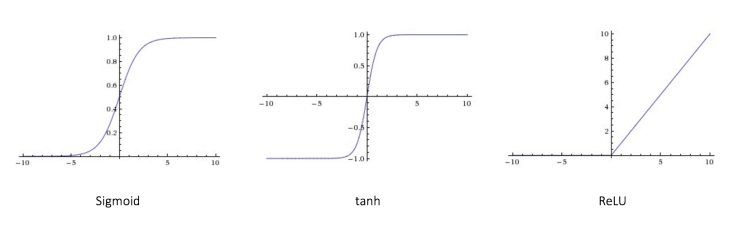
\includegraphics[width=0.9\textwidth]{Figures/factivacion.png}
	\caption{Funciones de activación \\ Fuente:  \href{https://ujjwalkarn.me/2016/08/09/quick-intro-neural-networks/}{\textit{https://ujjwalkarn.me}}}
	\label{activacion}
\end{figure} 

\subsection{Redes Neuronales Artificiales}
Las redes neuronales artificiales(ANN) toman la arquitectura del cerebro como inspiración para la construcción de sistemas inteligentes. Actualmente son la base para el desarrollo de la inteligencia artificial.\\
Una red neuronal está constituida por las uniones de neuronas.\\
En la figura 3.10 podemos ver la comparación entre una neurona biológica y un artificial etiquetadas con A y B respectivamente. Además observamos que las redes neuronales artificiales (etiqueta D) imitan el la unión biológicas de las neuronas o sinapsis(Etiqueta C).

\begin{figure}[H]
	\centering
	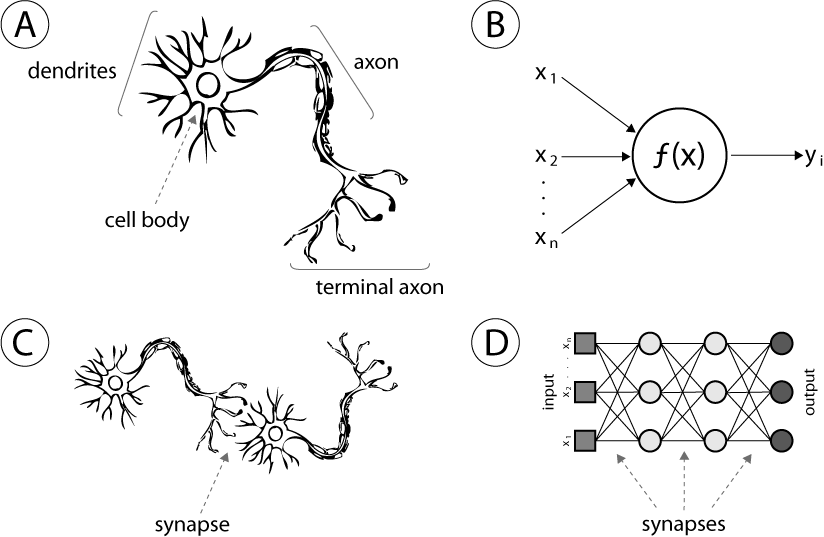
\includegraphics[width=0.8\textwidth]{Figures/ANN.png}
	\caption{Redes neuronales biológicas y artificiales \\ Fuente:  \href{https://medium.com/@ivanliljeqvist/the-essence-of-artificial-neural-networks-5de300c995d6}{\textit{https://medium.com}}}
	\label{neuronas}
\end{figure} 
\section{Redes Neuronales FeedFoward}
Estás redes fueron de las primeras y más simples. Contienen múltiples neuronas (nodos) ordenadas en capas de modo que los nodos en capas adyacentes se conectan. Cada una de estas conexiones poseen un peso asociado a dicha conexión.\\
En la figura 3.3 mostramos el esquema de Redes FeedFoward con sus distintas capas(layer).
\begin{figure}[H]
	\centering
	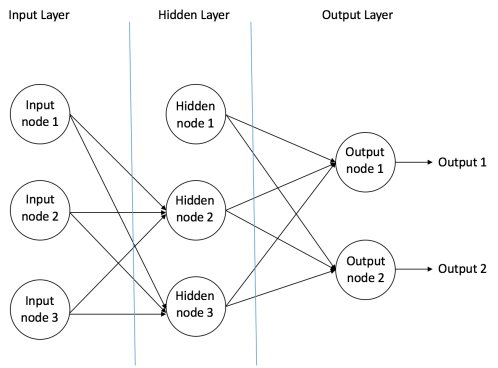
\includegraphics[width=0.5\textwidth]{Figures/esquemaff.png}
	\caption{Esquema de Redes Neuronales FeedFoward \\ Fuente:  \href{https://ujjwalkarn.me/2016/08/09/quick-intro-neural-networks/}{\textit{https://ujjwalkarn.me}}}
	\label{neuronasredes}
\end{figure} 
\begin{itemize}
	\item \textbf{Nodo de entrada(Input Node):} Proveen información a la red. En conjunto representan la capa de entrada, ningún calculo es realizado en esta capa solo se transfiere la información a la capa oculta.
	\item \textbf{Nodo Oculto(Hidden Node):} El trabajo de los nodos ocultos es calcular y transferir la información hacia a el nodo de salida. Una Red FeedFoward tiene solo una capa de entrada y una salida pero puede tener múltiples capas ocultas.
	\item \textbf{Output Node:}Su tarea principal es realizar cálculos y transferir la información fuera de la red.
\end{itemize}
En las Redes Neuronales FeedFoward, la información solo se propaga en una dirección hacia \textit{adelante} desde los nodos de entradas pasando por los nodos ocultos hacia los nodos de salida. No existen ciclos en este tipo de red.\\
Dentro de las redes neuronales FeedFoward tenemos algunos ejemplos:
\begin{itemize}
	\item \textbf{Perceptron Simple:} Es un red prealimentada simple que no posee capa oculta. Solo puede aprender de funciones lineales.
	\item \textbf{Perceptron Multicapas:} Esta red posee una o más capas ocultas. Este perceptron puede aprender de funciones no lineales.
	\item \textbf{Redes neuronales de convolución:} Este tipo de redes neuronal será explicada más adelante en el capítulo.
\end{itemize}
\subsection{Algoritmo de propagación hacia atrás}
El algoritmo de propagación hacia atrás trata de aprender de los errores, en el aprendizaje supervisado los conjuntos de entrenamiento se encuentran etiquetados. Por lo cual podemos sabemos la salida esperada. \\
El algoritmos se aplica de la siguiente forma:

\begin{enumerate}
	\item Se toma un ejemplo y se asignan pesos aleatorios a todas las conexiones de la red. Luego por medio de las conexiones y funciones de activación se calcula la salida en las capas ocultas y de salida.
	\item Se calcula el error total y se propagan estos errores hacia atrás a través de la red y se calcula la gradiente, luego se usan métodos como gradientes de descenso para ajustar los pesos y reducir el error en la capa de salida.
	\item Se repite el proceso con los otros ejemplos
\end{enumerate}
\begin{figure}[H]
	\centering
	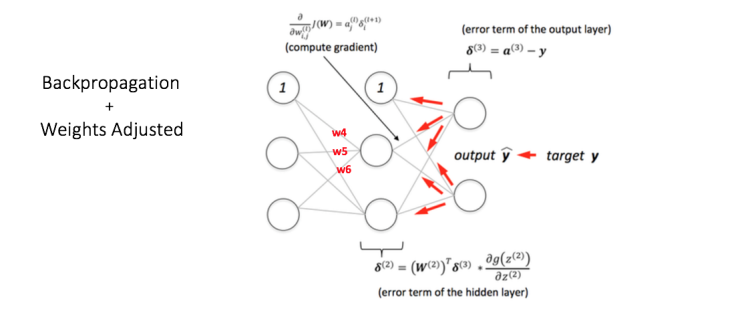
\includegraphics[width=0.9\textwidth]{Figures/backp.png}
	\caption{Propagación hacia atrás \\ Fuente:  \href{https://ujjwalkarn.me/2016/08/09/quick-intro-neural-networks/}{\textit{https://ujjwalkarn.me}}}
	\label{backpropagation}
\end{figure} 

\section{Redes Neuronales Convolucionales}
Las CNN son un tipo de Redes Neuronales FeedFoward que son especiales para procesar datos como imágenes las cuales son más difíciles de tratar en una red neuronal tradicional, como por ejemplo en el caso del perceptron multicapas.\\ El término \textit{convolucional} hace referencia a la operación lineal matemática usada. Las redes neuronales convolucionales usan esta operación para aprender de las características de mayor orden presente en los datos.
La primera CNN fue creada por Yann LeCun. Estas redes neuronales fueron inspiradas en la corteza visuales de los animales. Las células de la corteza visual, estas se activan para realizar tareas como el reconocimiento de patrones.\\  Entre sus usos más comunes tenemos el reconocimiento de imágenes y lenguaje natural.\\
\subsection{Estructura de una imagen}
Debido a que las redes neuronales convolucionales son usadas comúnmente con imágenes, es importante conocer cual es la estructura de una imagen y cómo es que la computadora comprende y utiliza esta información.\\
Las imágenes están constituidas por una sucesión de píxeles, podemos entender el pixel como la menor unidad homogénea en color de una imagen digital. Teniendo este concepto, podemos dividir la información de una imagen de la siguiente forma:
\begin{itemize}
	\item \textbf{Width}: El ancho de la imagen medido en pixeles
	\item \textbf{Height}: El alto de la imagen medida en pixeles.
	\item \textbf{Canales RGB}: Estos canales contiene la información de los colores y profundidad de una imagen. Este canal guarda la información en tres canales Red, Green y Blue.
\end{itemize}

\begin{figure}[H]
	\centering
	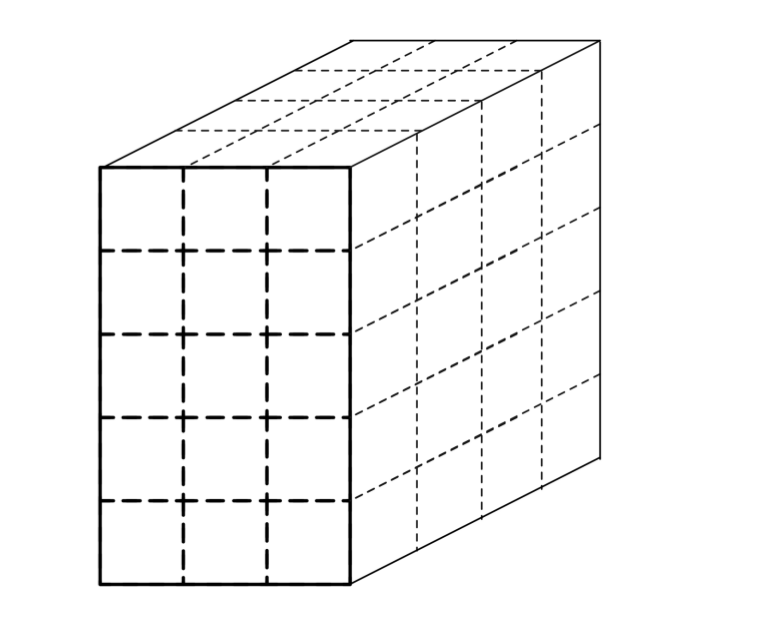
\includegraphics[width=0.7\textwidth]{Figures/image.png}
	\caption{Estructura de la imagen de entrada \\ Fuente:  \href{https://www.safaribooksonline.com/library/view/deep-learning/9781491924570/ch04.html}{\textit{Deep Learning by Adam Gibson, Josh Patterson}}}
	\label{image}
\end{figure} 

Teniendo en cuenta esta forma de dividir la información de una imagen podemos resaltar la ventaja de usar Redes convolucionales en lugar de usar una red neuronal multicapas.\\ Las redes multicapas toman un vector de una dimensión como entrada, si quisiéramos entrenar un perceptron multicapas con imágenes de 32x32 píxeles y con 3 canales RGB necesitaríamos crear 3072 pesos ($w_{i}$) para una sola neurona en la capa oculta. Esta generación excesiva de peso hace que la tarea resulte complicada usando redes multicapas.\\ De esta forma surge la idea de recurrir a un tiempo tipo de redes neuronales que faciliten la tarea sin consumir muchos recursos.
\subsection{Capas de una CNN}
Las redes neuronales convoluciones pueden ser dividas en distintas capas, cada una de ellas con una tarea específica para el tratamiento de la información. En esta sección describiremos cada una de estas capas.
\subsubsection{Input layer}
Esta capa es la encargada de cargar y almacenar la información de las imágenes para luego procesarlas en la red. Esta información contiene detalles de ancho, alto en píxeles y el número de canales de imagen. Las entradas de esta capa corresponden a la imagen vista en la figura 3.5.

\subsubsection{Convolutional layers}
Es una de las capas más importante en el diseño de las CNNs, esta capa es la encargada de transformar la entrada(imagen o convolución anterior) usando las conexiones de las neuronas en capas anteriores. 

Para entender más a fondo esta capa debemos definir la operación de \textit{convolución}.\\  La \textit{convolución} es una operación matemática que describe una regla de como fusionar 2 conjuntos de información.\textquotedblleft  Esta operación tiene importancia en campos como la matemática y la física debido que permite definir un puente entre el domino del espacio/tiempo y el dominio de la frecuencias a través del uso de la transformada de fourier.
La convolución toma una entrada, aplica un kernel de convolución y nos da un mapa de características como salida \textquotedblright \cite{book1} .\\
Las convoluciones son usadas principalmente como un detectores de características cuyas entradas son la capa de entrada u otra convolución.
En la figura 3.6 observamos la operación de convolución que por medio del uso de un kernel o filtro de convolución extrae características de la imagen, por ejemplo detalles como bordes de una imagen.\\ Haciendo analogía con los pesos en las redes neuronales convencionales, las redes convolucionales poseen el \textit{ filtro o kernel }, esto resulta beneficioso, ya que no se tendrá definir un peso para cada neurona.\\ El kernel de la figura 3.6 será desplazado a lo largo de las dimensiones espaciales. Durante el desplazamiento, el kernel se multiplicará por los datos de entrada dentro de su limite, produciendo una sola salida al mapa de características.
\begin{figure}[H]
	\centering
	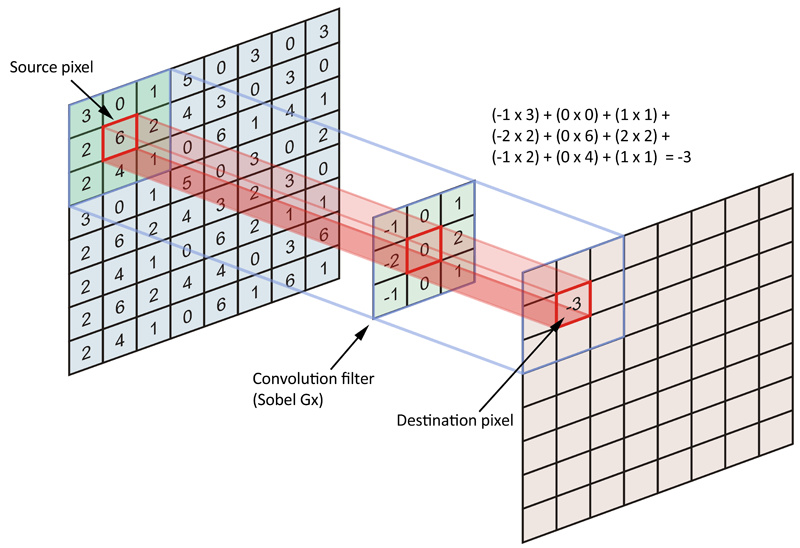
\includegraphics[width=0.8\textwidth]{Figures/convolucion.jpeg}
	\caption{Operacion de convolución \\ Fuente:  \href{http://openresearch.ai/t/network-in-network/39}{\textit{www.openresearch.ai}}}
	\label{convolucion}
\end{figure} 

Las capas convolucionales aplican transformaciones o funciones de activación al conjunto de entrada, luego el mapa de activación generado se apilará a lo largo de dimensión de profundidad para construir el volumen de salida.

\textbf{Componentes de la capa de convolución}.\\	\\
Las capas convolucionales poseen parámetros e hiperparámetros. La gradiente de descenso tiene la funcion de entrenar a estos parámetros de modo que las clases sean consistentes con las etiquetas en el conjunto de entrenamiento. Entre estos parámetros tenemos:
\textbf{Filtros}

Los filtros son una función que posee ancho(width) y alto (height) más pequeños que la entrada. Los filtros son aplicados a través de  del ancho y alto de la entrada, pero también pueden ser aplicados a lo largo de la profundidad.

\vspace{5cm}
\textbf{Hiperparámetros de una capa de convolución}.\\
A continuación veremos algunos hiperparámetros que determinan la disposición espacial y tamaño del volumen de salida de una capa convolucional.
\begin{itemize}
	\item \textbf{Filter size:} Cada filtro es pequeño con respecto al ancho(width) y alto(height) del la capa anterior. Por ejemplo podemos tener un filtro de tamaño $[5x5x3]$, lo representa 5 de ancho x 5 de alto x 3 de los canales RGB.
	\item \textbf{Output depth:} Este hiperparámetro controla el número de neuronas en la capa convolucional que están conectadas al mismo del volumen de entrada. Este parámetro puede ser elegido manualmente.
	\item \textbf{Stride:} Se encarga de configurar el tamaño de desplazamiento de la ventana de filtro. Cada filtro aplicado a la columna de entrada asignará más profundidad en el volumen de salida. Un stride grande creará un volumen de salida más grande y uno valor pequeño obtendrá un volumen menor.
	\item \textbf{Zero-padding:} Con este parámetro se puede controlar el volumen de salida. Es usado para mantener el tamaño espacial de entrada en la salida. 
\end{itemize}

\subsubsection{Pooling layers}
Este tipo de capas se encuentran entre las capas convolucionales. Se encarga de reducir el tamaño espacial(ancho,alto) de los datos de representación. Esta capa reduce la representación de los datos progresivamente a través de la red y ayuda a controlar el \textit{overfitting}.\\
Esta capa utiliza la operación \textit{max()} para cambiar el tamaño de los datos de entrada espacialmente, a esta operación se le conoce como max pooling. Esta funciona de siguiente forma toma un filtro de $n x n$, y la operación $max$ toma el mayor de los números en el área de filtro.\\ \\ Por ejemplo en caso tener una imagen de entrada $32 \times 32$ píxeles y se aplica un filtro de $2\times2$, como resultado obtendremos una salida de $16\times16$ píxeles. Esto reduce cada segmento de profundidad en el volumen de entrada por un factor de 2.

\subsubsection{Fully Connected Layers}

Esta capa se calcula el puntaje de las clases que usaremos como salida de red, esta será la encargada de reconocer a que clase pertenece una imagen de prueba de acuerdo a su puntaje o probabilidad. Las dimensiones del volumen de la salida son [1x1xN], donde el valor de N corresponde al número de clases de salida que se están evaluando. En el caso del MNIST (dataset para reconocimiento de dígitos), el valor de N es igual a 10, número que corresponde a los 10 dígitos distintos que posee el dataset($0, ... ,9$).\\
Esta capa tiene conexión entre todas sus neuronas y las de la capa anterior. Esta capa realiza las transformaciones del volumen de datos de entrada. Estas son funciones de activación en el volumen de entrada y los parámetros (pesos y bias de las neuronas).
\vspace{2cm}
\subsection{Arquitecturas conocidas}
Actualmente existen algunas arquitecturas de CNN ya diseñadas que son aplicadas para el trabajo de reconocimiento de imágenes.\\ El proyecto ImageNet, posee una gran base de datos de imágenes. Este proyecto realizá una competición llamada \textit{ImageNet Large Scale Visual Recognition Challenge (ILSVRC) } donde compiten distintos programas de software para detectar y clasificar objetos.\\ A continuación mostraremos algunas de las arquitecturas más importante de esta competencia:

\begin{itemize}
	\item \textbf{LeNet-5 (1998)} \textquotedblleft Arquitectura propuesta por LeCun, consiste 2 capas de convolución, activación  y capas pooling seguidas por a fully conected layer\textquotedblright \cite{WEBSITE:9}
	\vspace{1cm}
	\item \textbf{AlexNet (2012)} Fue propuesta por Alex Krizhevsky, esta arquitectura posee 5 capas de convolución seguida por 3 fully connected layers.
	\vspace{1cm}
	\item \textbf{VGGNet (2014)} Fue desarrollada para Sigmoyan y Zisserman para la competición ILSVRC. \textquotedblleft VGG consta de 16 capas convolucionales y es muy atractivo debido a su arquitectura uniforme. Consta de convoluciones de 3x3 y utiliza múltiples filtros \textquotedblright \cite{WEBSITE:10}	
\end{itemize}

\section{Redes Recurrentes}
Las redes neuronales recurrentes aparecieron en los años 1980s, actualmente se han desarrollado más estudios debido a la mejora de hardware. Son utilizadas principalmente para tratar con una información de secuencia, por ejemplo series de tiempo, audio, sentencia de oraciones, etc.\\ La principal diferencia de la redes con las redes neuronales feed-foward es que en las neuronas de las redes recurrentes las salidas regresan a la entrada de esta manera mantiene información de un estado anterior. Esto permite que nuestro modelo sea cambiante cada vez que este se alimente con una secuencia nueva.%%\subsubsection*{Características}

Dentro de una capa recurrente se tiene los siguientes tipos de conexiones :
\begin{itemize}
	\item  \textbf{Entrantes:} Son aquellas que emanan de la capa previa.
	\item  \textbf{Salientes:} Estas conexiones son dirigidas a todas las neuronas de las capas consecuentes.
	\item  \textbf{Recurrentes:} se encargan de propagar la información entre las neuronas de las misma capa.
\end{itemize}


\begin{figure}[H]
	\centering
	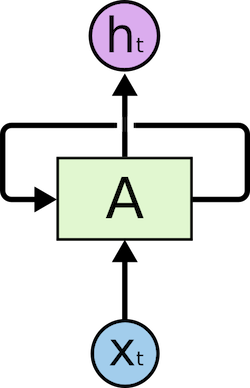
\includegraphics[width=0.3\textwidth]{Figures/rnn.png}
	\caption{Neurona Recurrente \\ Fuente:  \href{https://cdn-images-1.medium.com/max/960/1*XB5c4rTCSeFQrK0aFC5IVw.png}{\textit{https://medium.com}}}
	\label{}
\end{figure}

Es posible representar a la redes recurrentes como si fueran redes feed-fowards esto lo realizamos \textit{desenrrollando} la neurona como vemos en la figura 3.8 el $x_{t}$ representa un estado final de esta forma podemos representar la red como un conjunto de estados a través de un lapso de tiempo. En esta forma las técnicas de backpropagation pueden ser usadas en la redes recurrentes.

\begin{figure}[H]
	\centering
	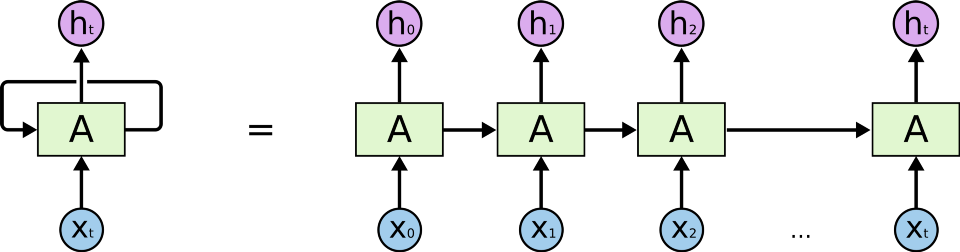
\includegraphics[width=0.9\textwidth]{Figures/rnn2.png}
	\caption{Versión desenrollada \\ Fuente:  \href{https://towardsdatascience.com/introduction-to-recurrent-neural-network-27202c3945f3}{\textit{https://towardsdatascience.com}}}
	\label{}
\end{figure}
\newpage
\subsection{Propagación hacia atrás través del tiempo(BPTT)}

Las redes neuronales feedfoward, la propagación hacia atrás se encarga de transmitir el error de la salida hacia a las capas ocultas asignados a los pesos(w) responsabilidad del error general mediante el uso de la derivada parcial $\frac{ { \partial } E } { \partial w }$. En estas redes es común usar la propagación hacia atrás debido a que el par entrada salida posee un tamaño fijo situación que no ocurre con las secuencia de datos.\\
 Las redes neuronales recurrentes utilizan una extensión de la propagación hacia atrás llamada \textit{Propagación hacia atrás a través del tiempo}, o BPTT  por sus siglas en inglés, la cual se aplica para secuencia de datos.
Este algoritmo consta de los siguiente pasos:
\begin{itemize}
	\item Dado unos lapsos de tiempo entre la entrada y la salida de la red.
	\item Se desenrolla la red(Ver Figura 3.8) , calcula y acumulada los errores de cada lapso de tiempo.
	\item Enrolla la red y actualiza los pesos para reducir el error.
	
\end{itemize}

\textquotedblleft Si la secuencia de datos consta de 1000 lapsos de tiempo, este será el número de derivadas requeridas para una simple actualización \textquotedblright \cite{WEBSITE:20}

\begin{figure}[H]
	\centering
	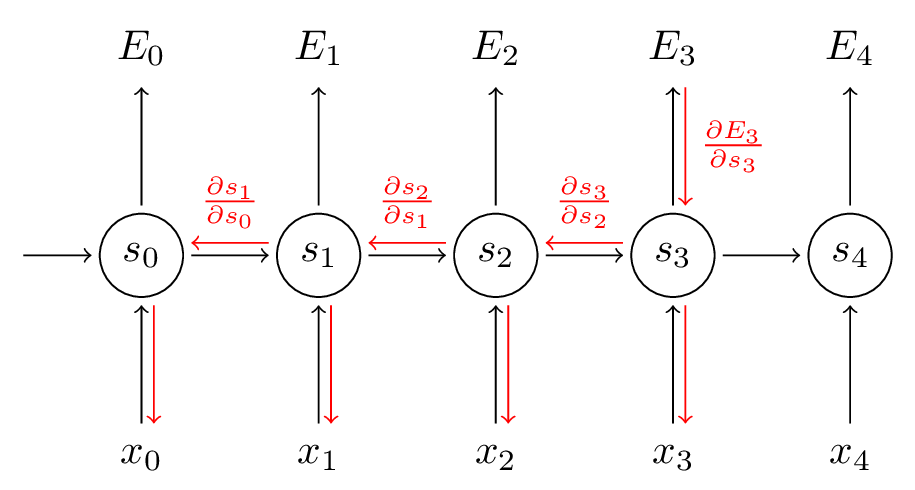
\includegraphics[width=0.8\textwidth]{Figures/BPTT1.png}
	\caption{BPTT \\ Fuente:  \href{http://www.wildml.com/2015/10/recurrent-neural-networks-tutorial-part-3-backpropagation-through-time-and-vanishing-gradients/}{\textit{http://www.wildml.com}}}
	\label{}
\end{figure}

En este esquema de básico de redes neuronales recurrentes utilizamos la función de activación softmax para calcular los valores de la celda y utilizamos pesos($U,W,V$) de esta forma tenemos que:
\begin{equation}
	\label{ST}
	\begin{aligned}
	s_{t}&=\tanh(Ux_{t}+Ws_{t-1})\\
	\hat{y}_{t}&=softmax(Vs_{t})
	\end{aligned}
\end{equation}
Donde $s_{t}$ son los valores de la celda y $\hat{y}_{t}$ es la predicción. A continuación calcularemos el error de nuestra red utilizando el valor de la predicción $\hat{y}_{t}$ y el valor real $y_{t}$.
\begin{equation}
	\label{STs}
	\begin{aligned}
		E_{t}(y_{t},\hat{y_{t}})&=y_{t}logy_{t}\\
		E_{t}(y,\hat{y})&=\sum_{t}{E_{t}(y_{t},\hat{y_{t}}}\\
	\end{aligned}
\end{equation}
Nuestro objetivo será ajustar los pesos ($U,W,V$) por lo cual usaremos la gradiente de descenso con respecto a los pesos los cuales serán calculados en la ecuación 3.4.

\begin{equation}
\label{Ts}
\begin{aligned}
	\frac{\partial E}{\partial W}&=\sum_{t}{\frac{\partial E_{t}}{\partial W}}
\end{aligned}
\end{equation}
Para calcula esta gradiente haremos uso de la regla de la cadena para simplificar los cálculos usaremos un ejemplo el $E_{t}$ para $t=2$.


\begin{equation}
\label{Tsfs}
	\begin{aligned}
	\frac{\partial E_{2}}{\partial V}&=\frac{\partial E_{2}}{\partial \hat{y_{2}}} \frac{\partial \hat{y_{2}}}{\partial V}\\
	\frac{\partial E_{2}}{\partial V}&=\frac{\partial E_{2}}{\partial \hat{y_{2}}} \frac{\partial \hat{y_{2}}}{\partial z_{2}} \frac{\partial \hat{z_{2}}}{\partial V}\\
	\frac{\partial E_{2}}{\partial V}&=(\hat{y_{2}}-y_{2})\otimes s_{3}
	\end{aligned}
\end{equation}
Donde $s_{2}=Vs_{3}$ ahora calcularemos para W como $s_{2}=tanh(Ux_{t}+ Ws_{1})$
Al derivar obtenemos la ecuación 3.6 luego se sumarán las contribuciones en cada lapso de tiempo.
\begin{equation}
\label{TsSfs}
	\begin{aligned}
		\frac{\partial E_{2}}{\partial W}&=\frac{\partial E_{2}}{\partial \hat{y_{2}}} \frac{\partial \hat{y_{2}}}{\partial s_{2}} \frac{\partial \hat{s_{2}}}{\partial s_{k}} \frac{\partial s_{k}}{\partial W}
	\end{aligned}
\end{equation}


\subsection{Propagación dinámica hacia atrás (DBP)}
Este algoritmo fue propuesto por Pineda\cite{PINEDA} en 1987. Este tipo de redes neuronales son utilizados a las redes neuronales dinámica, la cual esta representada por la ecuación no lineal de tiempo discreto mostrará en la ecuación 3.7


\begin{equation}
\label{ECUATION}
\begin{aligned}
\left\lbrace
\begin{array}{ll}
x(k+1)=f(x(k),W,\theta) \\
y(k)= h(x(k))
\end{array}
\right.
\end{aligned}
\end{equation}

\begin{itemize}
	\item $x=[x_{1}...,x_{n}]^{T}$: Vector de estado de la red dinámica
	\item  $x_{i}$ : estado interno de la neurona $i$
	\item  $W=[w_{ij}]_{nxn}$: Matriz de valores de pesos.
	\item $\theta=[\theta_{1}...,\theta_{n}]^{T}$: vector somático.
	\item $f:R^{n}\times R^{n\times n}\times R^{n} \rightarrow R^{n}$ función continua y diferenciable.
	\item $h(x):R^{n} \rightarrow R^{m}$ función continua y diferenciable. 	
\end{itemize}



Para el caso de redes recurrentes se tienen conexiones hacia adelante y hacia atrás entre las capas y las neuronas. Ahora los pesos $w_{ij}$ representa la conexión sinaptica entre la i-ésima  y j-ésima y $\theta_{i}$ umbral en la i-ésima neurona.


\begin{equation}
\label{ECUATIONs}
\begin{aligned}
\left\lbrace
\begin{array}{ll}
x_{i}(k+1)=f_{i}(x(k),w_{i},\theta_{i}) \\
y(k)= h(x(k))
\end{array}
\right.
\end{aligned}
\end{equation}
Donde :
\begin{equation}
W=		
\begin{bmatrix}
	w_{11} & w_{12} & w_{13} & \dots  & w_{1n} \\
	w_{21} & w_{22} & w_{23} & \dots  & w_{2n} \\
	\vdots & \vdots & \vdots & \ddots & \vdots \\
	w_{n1} & w_{n2} & w_{n3} & \dots  & w_{nn}
\end{bmatrix}
=
\begin{bmatrix}
w_{1}^{T} \\
w_{2}^{T} \\
\vdots \\
w_{d}^{T}
\end{bmatrix}
\end{equation}

\begin{equation}
w_{i}=		
\begin{bmatrix}
	w_{i1}  \\
	w_{i2}  \\
	\vdots  \\
	w_{in} 
\end{bmatrix}
i=1,2 ...., n
\end{equation}

La ecuación 3.7 nos muestra que el comportamiento dinámico de la neurona depende los pesos ($w_{ij}$) y el parámetro $\theta_{i}$
Dado $t=[t_{1},...,t_{m}]^{T}$ un valor objetivo de nuestra red y nuestro propósito es encontrar los valores de pesos adecuados para estimar $ t=h(x^{f})$ . De esta forma podemos definir el error en la ecuación 3.11 .
\begin{equation}
E= \frac{1}{2} \sum_{l=1}^{m}[t_{l}-h_{l}(x^{f})]^{2}=\frac{1}{2}\sum(J_{l}^{f})^{2}
\end{equation}
Donde $J_{l}^{f}-t_{l}-h_{l}(x^{f})$ 

A continuación veremos como se actualizarán los parámetros $w_{ij}$  y $\theta_{i}$ usando tasa de aprendizaje $\eta_{w}$ y $\eta_{\theta}$ respectivamente.

\begin{equation}
	\begin{aligned}
	\bigtriangleup w_{ij}&=-\eta_{w}\frac{\partial E}{\partial w_{ij}} \\
	&=\eta_{w} \sum_{p=1}^{n} \sum_{l=1}^{m}[t_{l}-h_{l}(x^f)]\frac{\partial h_{l}(x^f)}{\partial x_{p}^f} \frac{\partial x_{p}^f}{\partial w_{ij}}\\
	&=\eta_{w} \sum_{p=1}^{n} \sum_{l=1}^{m}J_{l}^{f}\frac{\partial h_{l}(x^f)}{\partial x_{p}^f} \frac{\partial x_{p}^f}{\partial w_{ij}}
	\end{aligned}
\end{equation}

\begin{equation}
\begin{aligned}
\bigtriangleup \theta_{i}&=-\eta_{\theta}\frac{\partial E}{\partial \theta_{i}} \\
&=\eta_{\theta} \sum_{p=1}^{n} \sum_{l=1}^{m}[t_{l}-h_{l}(x^f)]\frac{\partial h_{l}(x^f)}{\partial x_{p}^f} \frac{\partial x_{p}^f}{\partial \theta_{i}}\\
&=\eta_{\theta} \sum_{p=1}^{n} \sum_{l=1}^{m}J_{l}^{f}\frac{\partial h_{l}(x^f)}{\partial x_{p}^f} \frac{\partial x_{p}^f}{\partial \theta_{i}}
\end{aligned}
\end{equation}

Derivando las ecuaciones 3.12 y 3.13
\begin{equation}
\begin{aligned}
\bigtriangleup w_{ij}&=-\eta_{w}z_{i}^f \frac{\partial f_{i}(x^f,w_{i},\theta_{i})}{\partial w_{ij}}\\
\bigtriangleup \theta_{i}&=-\eta_{\theta}z_{i}^{f}\frac{\partial f_{i}(x^f,w_{i},\theta_{i})}{\partial \theta_{i}} 
\end{aligned}
\end{equation}

Donde $z_{i}^f$ esta determinada por la siguiente ecuación:

\begin{equation}
\begin{aligned}
z_{i}^f =\sum_{p=1}^{n} \frac{\partial f_{p}}{\partial x_{i}^f}z_{p}^{f} + \sum_{l=1}^{m} J_{l}^f \frac{\partial h_{l}(x^f)}{\partial x_{i}^f}
\end{aligned}
\end{equation}
\newpage
\textquotedblleft Un algoritmo de propagación dinámica hacia atrás es utilizado para entrenar la red en configuraciones de bucle cerrado, cuando existe una ruta de retroalimentación entre la salida de la sección de filtro digital y las entradas a la red neuronal. \textquotedblright \cite{DBP}
\subsection{Desaparición de la gradiente}
Las redes recurrentes ofrecen una gran ventaja al manejar \textit{secuencias de datos} pero el trabajar con este tipo de datos también pueden repercutir en un problema conocido como la desaparición de la gradiente, o \textit{Vanishing Gradient}, el cual es una de la principales dificultades en las redes recurrentes.\\
 La gradiente de descenso nos permite actualizar los valores de nuestros pesos para que nuestra red continué aprendiendo, pero si esta gradiente desaparece, debido a que toma un valor pequeño, nuestra red deja de aprender en términos sencillos en esto consiste el problema de \textit{desaparición de gradiente}.

Dado que en la propagación hacia atrás se calcula la gradiente usando la regla de la cadena podemos suponer que usamos la función sigmoid de la figura 3.9 notamos que su derivada para valores positivos y negativos grandes toma el valor de 0 lo que producirá que la gradiente desaparezca y nuestra red deje de aprender al no poder actualizar.

Entre la soluciones para este problema se encuentran usar otras funciones de activación como Relu o Elu, también se pueden usar métodos de normalización para los batchs.
\begin{figure}[H]
	\centering
	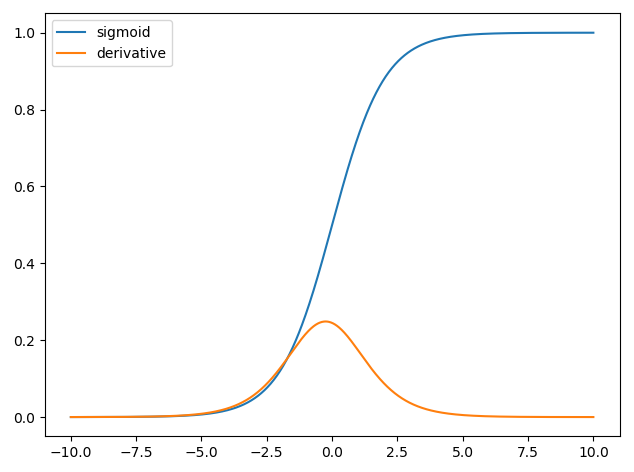
\includegraphics[width=0.5\textwidth]{Figures/sigmoid.png}
	\caption{Función sigmoid y su derivada \\ Fuente:  \href{https://cdn-images-1.medium.com/max/960/1*XB5c4rTCSeFQrK0aFC5IVw.png}{\textit{https://medium.com}}}
	\label{}
\end{figure}

\subsection{Long Short Term Memory (LSTM)}

LSTM es un tipo de red neuronal recurrente que fue propuesto por Sepp Hochreiter y Jurgen Schmidhuber.\cite{LSTM} para aprovechar las ventajas de las redes recurrentes y combatir el problema de la desaparición de gradiente.\\ En la redes recurrentes se trasmite la información pero ha medida que transcurre el tiempo están son olvidadas, a esto se le llamó el \textit{problema de las dependencias a largo plazo}. Las LSTM buscan solucionar este problema, por lo cual estas se encargan de transmitir la información y \textit{recordarla} mientras los lapsos de tiempo pasan imitando la \textit{capacidad de la memoria humana para recordar.}


\begin{figure}[H]
	\centering
	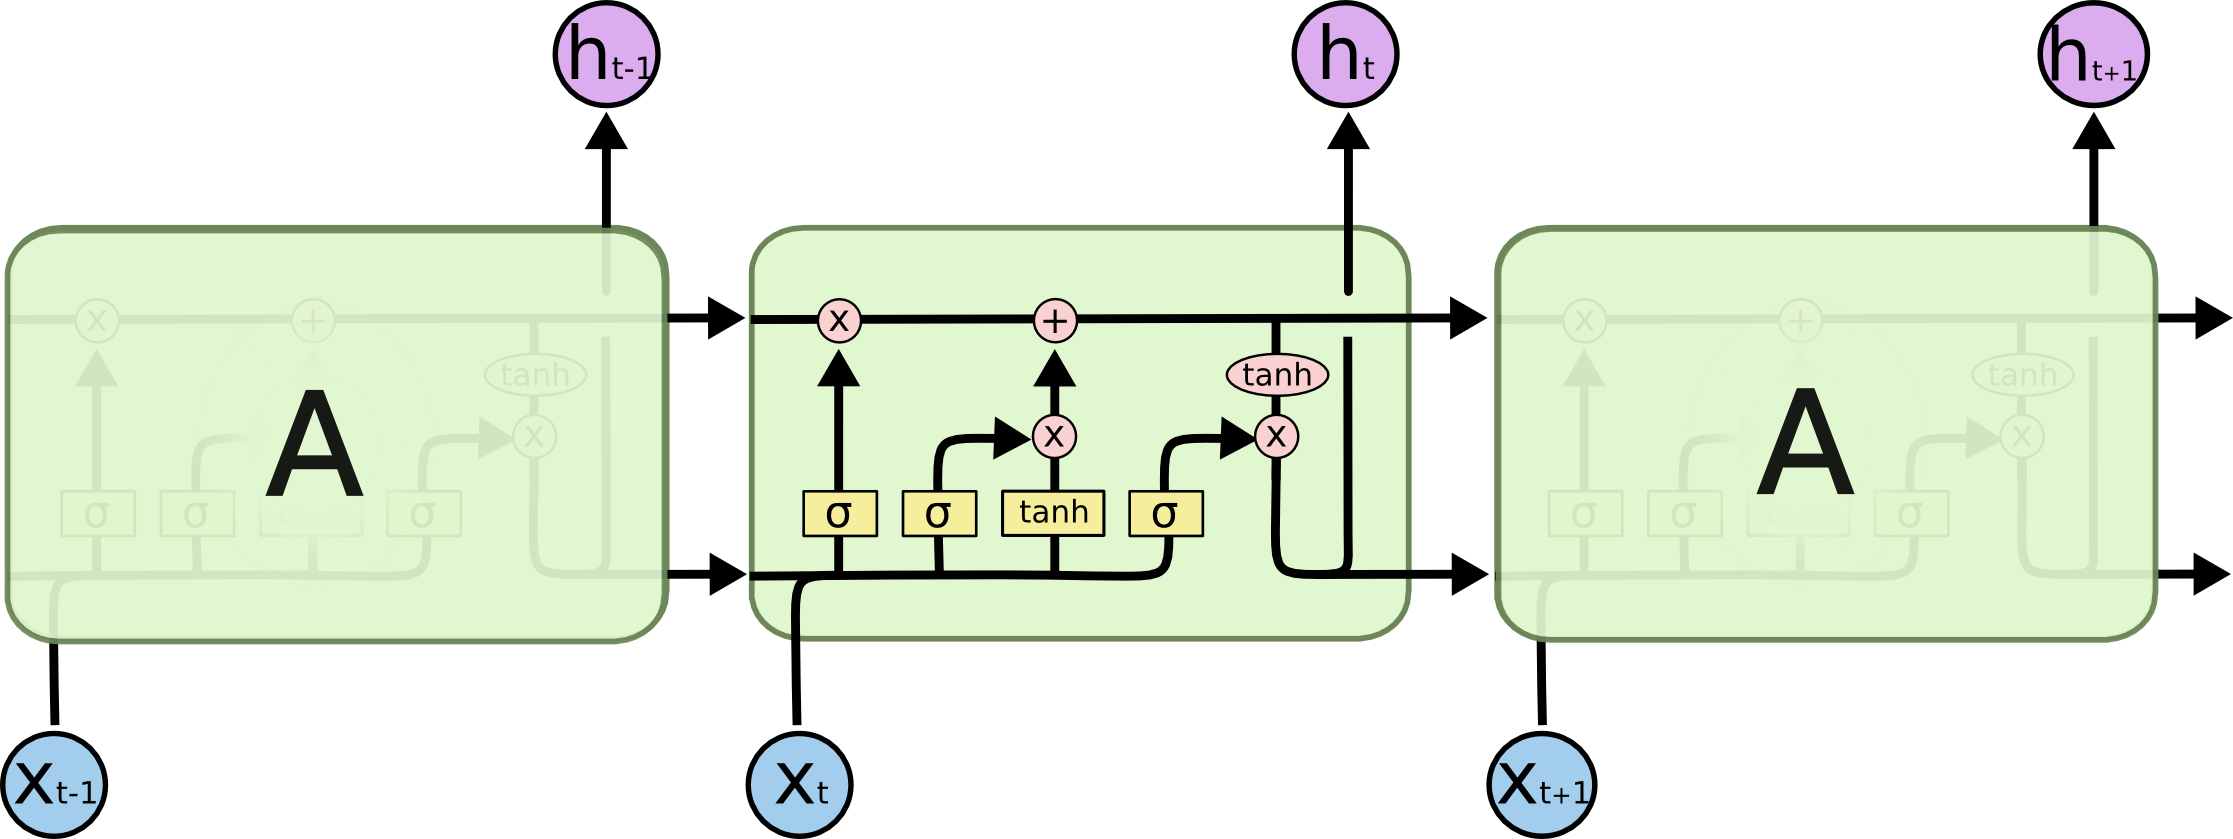
\includegraphics[width=0.8\textwidth]{Figures/LSTM-chain.png}
	\caption{Estructura en cadena \\ Fuente:  \href{http://colah.github.io/posts/2015-08-Understanding-LSTMs/}{\textit{http://colah.github.io}}}
	\label{}
\end{figure}

En la siguiente figura observamos el esquema de una unidad, o neurona, de LSTM y estudiaremos su comportamiento.
\begin{figure}[H]
	\centering
	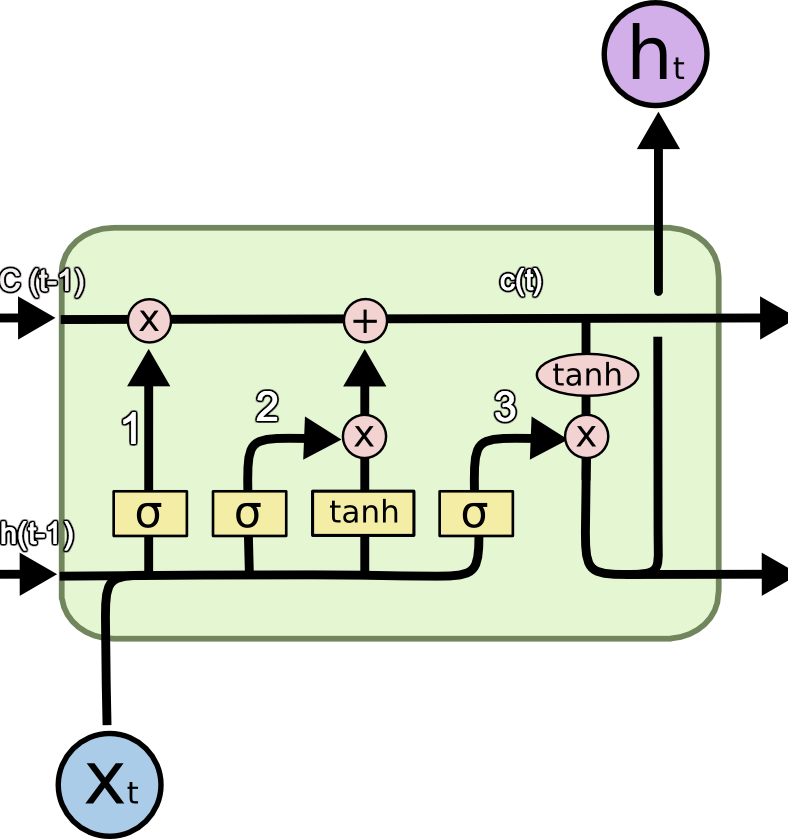
\includegraphics[width=0.4\textwidth]{Figures/LSTM.png}
	\caption{Unidad de LSTM \\ Fuente:  \href{https://towardsdatascience.com/understanding-lstm-and-its-quick-implementation-in-keras-for-sentiment-analysis-af410fd85b47g}{\textit{https://towardsdatascience.com}}}
	\label{}
\end{figure}

\begin{itemize}
	\item $X_{t}$: entrada actual
	\item $\sigma$: capa sigmoid
	\item $tanh$: capa tanh
	\item $h_{t-1}$: salidas de la última unidad.
	\item $C_{t-1}$: memoria de la última unidad.
	\item $h_{t}$: salida actual.
	\item $C_{t}$: memoria actualizada
	
\end{itemize}


Principalmente la idea de LSTM gira entorno a las celdas de estado  $c_{t}$, esta será la encargada de añadir nueva información o removerla si ya no es necesaria.

\begin{figure}[H]
	\centering
	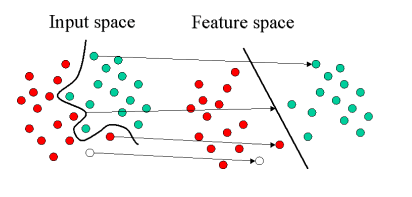
\includegraphics[width=1\textwidth]{Figures/kernel.png}
	\caption{celda de estado \\ Fuente:  \href{http://colah.github.io/posts/2015-08-Understanding-LSTMs/}{\textit{http://colah.github.io}}}
	\label{}
\end{figure}

El valor de la celda de estado($C_{t}$) y la salida($h_{t}$) :
\begin{enumerate}
	\item  Nuestro LSTM decidirá que información será desechada de nuestra célula de estado. Esta decisión utilizará una capa sigmoidal llamada \textit{forget gate layer} la cual genera un número entre 0 y 1, lo cual definirá la cantidad de información que mantendrá.
	\begin{figure}[H]
		\centering
		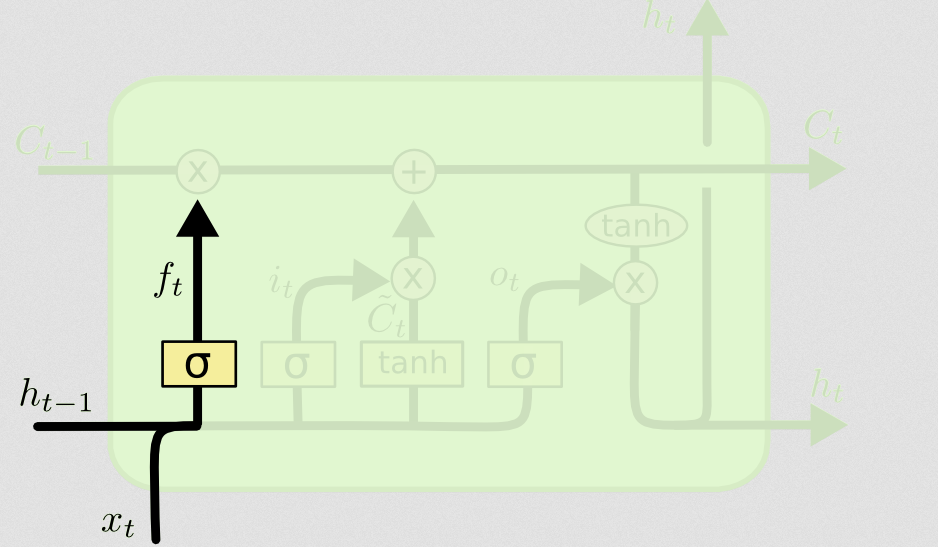
\includegraphics[width=0.75\textwidth]{Figures/forgetay.png}
		\caption{capa sigmoidal \\ Fuente:  \href{http://colah.github.io/posts/2015-08-Understanding-LSTMs/}{\textit{http://colah.github.io}}}
		\label{}
	\end{figure}
			\begin{equation}
				\label{forget layer}
				\begin{aligned}
				f_{t}&=\sigma(W_{t}\cdot[h_{t-1},x_{t}]+b_{f})
				\end{aligned}
			\end{equation}
	\item Una vez que se ha olvidado es importante es aceptar nueva información y almacenarla. Esto será realizado en los siguientes pasos.
	\begin{enumerate}
		\item Una capa sigmoid llamada \textit{input gate layer} decide que valores serán actualizados($i_{t}$).

	

		\item Una capa tanh crea un vector de valores posibles, o valores candidatos, $\hat{C}_{t}$ .
		\begin{figure}[H]
			\centering
			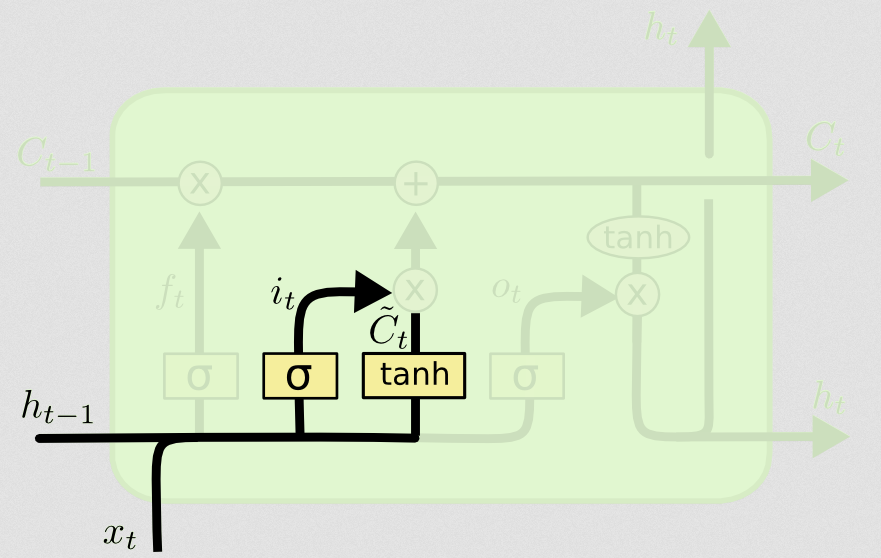
\includegraphics[width=0.75\textwidth]{Figures/forgetay2.png}
			\caption{capa tanh \\ Fuente:  \href{http://colah.github.io/posts/2015-08-Understanding-LSTMs/}{\textit{http://colah.github.io}}}
			\label{}
		\end{figure}
		\begin{equation}
			\label{forget layer}
			\begin{aligned}
			i_{t}&=\sigma(W_{i}\cdot[h_{t-1},x_{t}]+b_{i})\\
			\hat{C}_{t}&=\sigma(W_{C}\cdot[h_{t-1},x_{t}]+b_{C})
			\end{aligned}
			\end{equation}
		\item Finalmente se combinan ambos para actualizar la celda de estado.
		\begin{figure}[H]
			\centering
			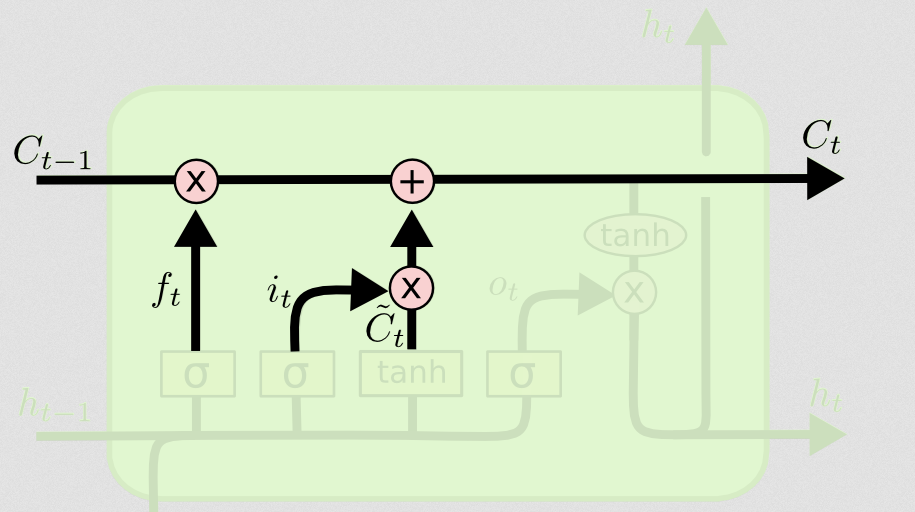
\includegraphics[width=0.6\textwidth]{Figures/LSTM8.png}
			\caption{Actualización del $C_{t}$ \\ Fuente:  \href{http://colah.github.io/posts/2015-08-Understanding-LSTMs/}{\textit{http://colah.github.io}}}
			\label{}
		\end{figure}
		\begin{equation}
			\label{ctlayer}
			\begin{aligned}
				C_{t}&=f_{t}\ast C_{t-1} + i_{t}\ast \hat{C}_{t}
		    \end{aligned}
		\end{equation}
	\end{enumerate}
\item Finalmente para obtener la salida de este módulo $C_{t}$
		\begin{figure}[H]
	\centering
	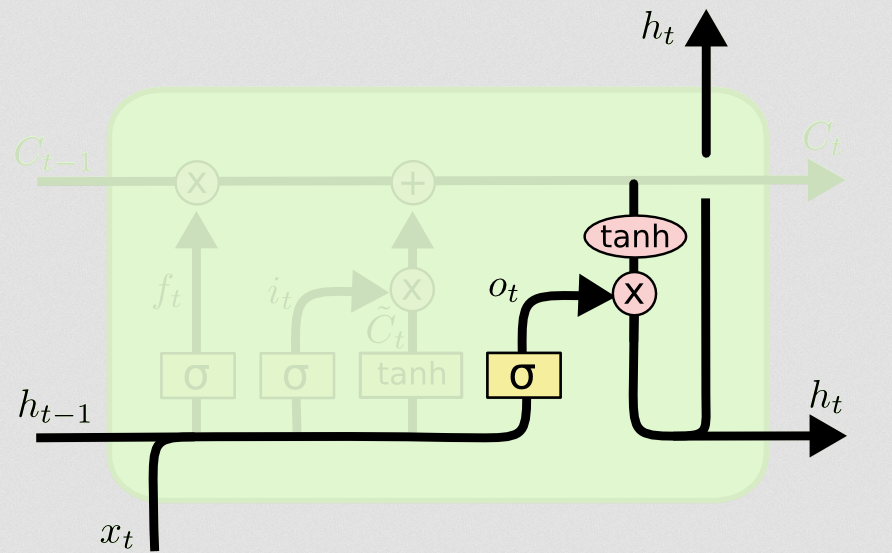
\includegraphics[width=0.75\textwidth]{Figures/LSTM9.png}
	\caption{Calculo del $h_{t}$ \\ Fuente:  \href{http://colah.github.io/posts/2015-08-Understanding-LSTMs/}{\textit{http://colah.github.io}}}
	\label{}
\end{figure}
		\begin{equation}
			\label{ht}
			\begin{aligned}
				o_{t}&=\sigma(W_{o}[h_{t-1},x_{t}]+b_{o})\\
				h_{t}&=o_{t}\ast \tanh(C_{t})
			\end{aligned}
		\end{equation}
\end{enumerate}

Una variante de las redes recurrentes son las redes recurrentes bidireccionales, la cual consiste en aprender de una secuencia de datos en 2 direcciones siguiendo lapsos de tiempo de la secuencia hacia adelante y atrás. Al capturar la información de la secuencia invertida nos permite mejorar nuestra predicción.	\textquotedblleft Para superar las limitaciones de una RNN regular proponemos un modelo bidireccional de redes recurrentes(BRNN) la cual puede ser entrenada con la información de entrada en el pasado y en el futuro de un marco especifico de tiempo \textquotedblright \cite{BRNN}


%%%
%%\begin{figure}[H]
%%\centering
%%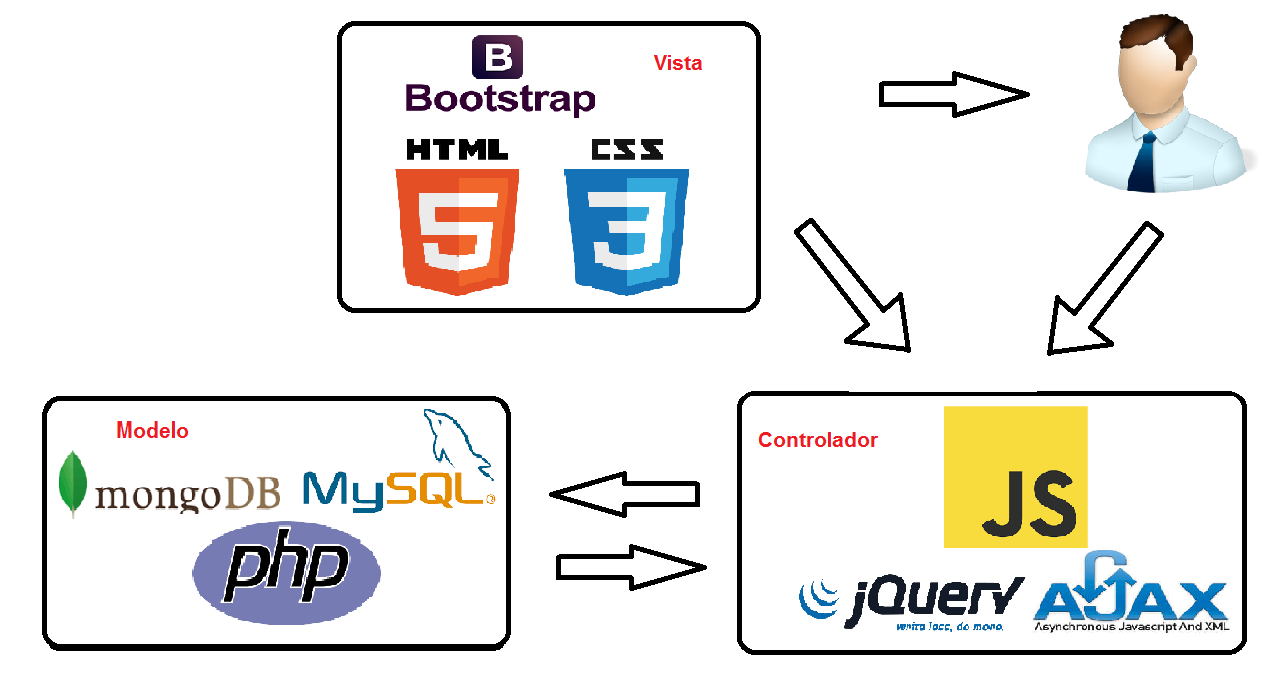
\includegraphics[width=0.9\textwidth]{Figures/mvc.png}
%%\caption{Modelo-Vista-Conrolador}
%%\label{MVC}
%%\end{figure}




%\newpage
$\ $
%\thispagestyle{empty} % para que no se numere esta pagina
\chapter{Procesamiento señal de voz}
En este capítulo conoceremos más acerca del procedimiento para procesar la señal de voz, además repasaremos algunos conceptos previos para entender en procesamiento y luego introduciremos 2 conceptos importantes \textit{Extracción de características y la coincidencia de patrones.}

\section{Conceptos previos}
\subsection{Voz}
Los seres humanos diariamente nos comunicamos por medio del habla utilizando nuestras voces somos capaces de transferir información en forma de \textit{ondas sonoras}.\\ Estas ondas transmiten una gran cantidad de información usando el aire como medio de transmisión.
Las propiedades como variaciones en amplitud al empezar o finalizar una palabra varían en el transcurso del tiempo, por lo cual es importante analizar segmentos de tiempo donde estas propiedades se mantengan aisladas de esta manera nos aseguramos que la señal de voz no cambie.
\subsection{Audios}
Los audios son un tipo de \textit{datos no estructurados}, es decir datos que no se encuentran en algún tipo de estructura de datos, estos tipos de datos son los que más se encuentran el mundo real como imágenes y audio. Una características de estos es que son complejos en su recolección y preparación para la realización de un análisis.\\ El audio puede capturarse mediante la grabación de nuestro entorno pero para que este audio sea entendido por las computadoras necesita un formato adecuado como: wav, mp3 y wma. \\
Debido a que el sonido es una señal de onda podemos analizar y obtener valores numéricos de este. En la figura 4.1 observamos una onda de la cual obtenemos valores almacenando las alturas de puntos equidistantes de esta forma guardamos información de esta onda.
\begin{figure}[H]
	\centering
	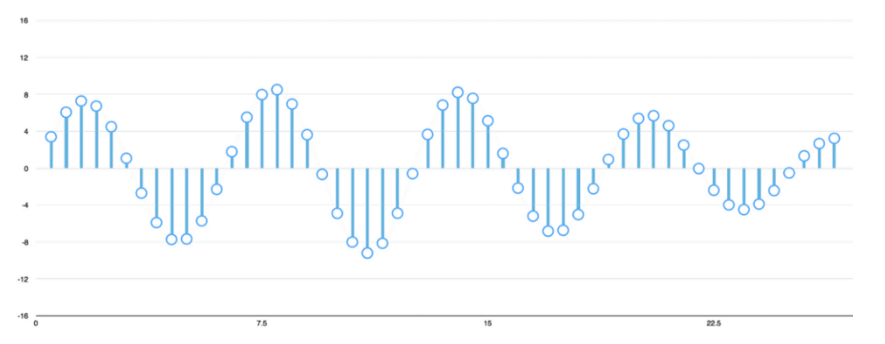
\includegraphics[width=0.9\textwidth]{Figures/onda.png}
	\caption{Onda de sonido \\ Fuente:  \href{https://medium.com/@venkateshpnk22/how-to-convert-your-speech-voice-to-text-data-1b2686099260}{\textit{https://medium.com}}}
	\label{onda}
\end{figure} 
\subsection{Espectro de frecuencias}
Consiste en la distribución de amplitudes para un valor dado de frecuencia de un fenómeno ondulatorio en este caso ondas sonoras.
\begin{figure}[H]
	\centering
	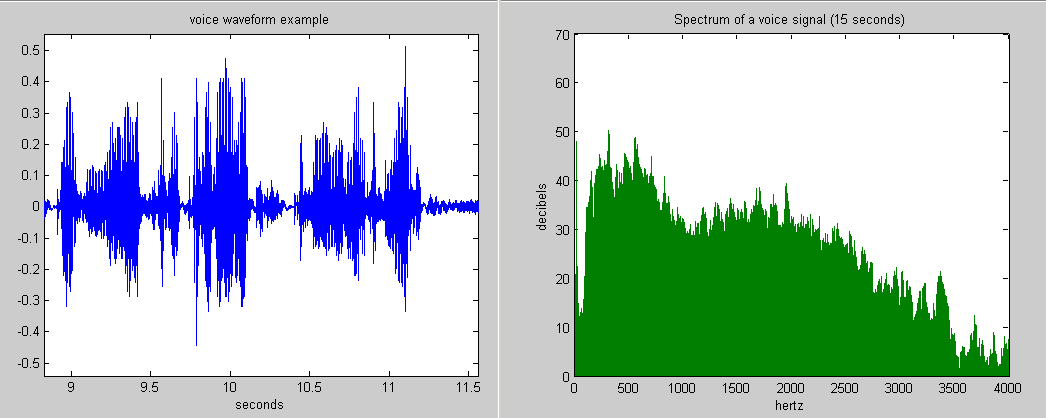
\includegraphics[width=0.8\textwidth]{Figures/espectro.png}
	\caption{señal de voz y su espectro asociado\\ Fuente:  \href{https://www.finaltest.com.mx/product-p/art-03.htm}{\textit{https://www.finaltest.com.mx}}}
	\label{señal}
\end{figure} 

\subsection{Escala mel}
Es una escala psicoacústica propuesta por Stevens, Volkman y Newman. Esta escala es muy importante debido a que la representación más usada en las señales de voz.
\begin{figure}[H]
	\centering
	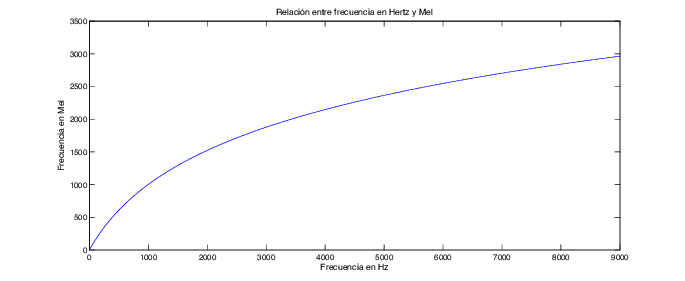
\includegraphics[width=0.8\textwidth]{Figures/escala_mel.png}
	\caption{Relación escala mel - Frecuencia\\ Fuente:  \href{https://www.researchgate.net/figure/Relacion-entre-frecuencia-en-Hz-eje-x-y-en-escala-Mel-eje-y_fig2_312041038}{\textit{https://www.researchgate.net}}}
	\label{mel}
\end{figure} 
\begin{equation}
	\label{STg}
	\begin{aligned}
	m=1127.01048\log_{e}(1+f/700))
	\end{aligned}
\end{equation}
\subsection{Dominio de tiempo}
Este dominio permite obtener la amplitud en un instante de tiempo dado existen dominio de tiempo discretos y continuos.
\subsection{Dominio de frecuencia}
Este dominio permite representar a nuestra frecuencia de onda como un par de amplitud y valores de la fase. Para señales periódicas se relaciona con series de fourier y para señales no periódicas se relaciona con la transformada de fourier.
\begin{figure}[H]
	\centering
	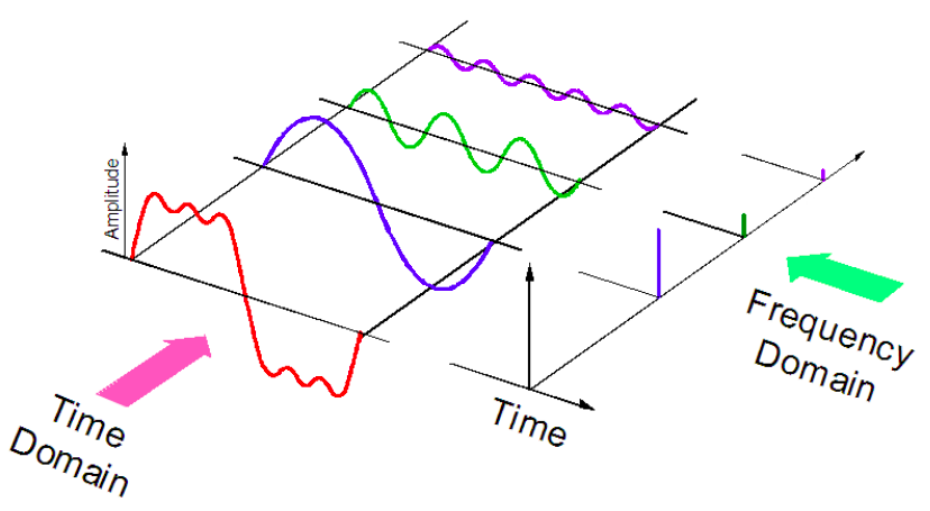
\includegraphics[width=0.6\textwidth]{Figures/audio_signal.png}
	\caption{Dominios de tiempo y frecuencia de dominio\\ Fuente:  \href{https://medium.com/@venkateshpnk22/how-to-convert-your-speech-voice-to-text-data-1b2686099260}{\textit{https://medium.com}}}
	\label{onda}
\end{figure} 


\section{Proceso de extracción de características}

También conocido como análisis de la señal de voz este proceso retené la información necesaria de la voz y elimina los datos redundantes y no necesarios. Este proceso es uno de los más importantes debido a que se transforma la señal en una forma adecuada para los modelos de clasificación. 
\subsection{Etapas del proceso de extracción de carácterísticas}

El proceso de extracción de características puede ser divido en 3 etapas o subprocesos.
\subsubsection{1. Análisis Espectral}
El análisis espectral consiste en descomponer algo complejo en parte o identificar propiedades de la muestra analizada.
Cuando tratamos con una seña de voz esta es variable en el tiempo, por tanto podemos identificar sus características en función a la actividad espectral. El análisis espectral puede ser realizado usando los siguientes métodos:
\begin{itemize}
	\item \textbf{Banco de filtros digitales\\}
	Es un sistema que divide una señal de entrada $x(n)$ en un conjunto de señales $x_{1},x_{2},..$ donde cada una corresponde a una región del espectro de $x(n)$.
	\item \textbf{Transformada de fourier\\}
	Dada una señal aperiódica discreta en el tiempo $x(n)$ definimos la transformada discreta de Fourier como:
	\begin{equation}
	\label{STgl}
	\begin{aligned}
		X(k)=\sum_{n=0}^{N-1}x(n)\exp^{-j2\pi k \frac{n}{N}} k=0, ..., N-1
	\end{aligned}
	\end{equation}
	Esta transformada es calculada por la transformada rápida de Fourier, esta tiene el objetivo de encontrar los componente de la frecuencia en una señal ruidosa dentro de su dominio de frecuencia.
	\item \textbf{Predicción Lineal\\}
	La predicción Lineal o LP, es una técnica para modelar el espectro de la señal de voz por medio de los espectros de todos los polos. \textquotedblleft El método permite la conformación espectral arbitraria en el dominio de la frecuencia y el modelado de espectros continuos y discretos. \textquotedblright \cite{LP}
\end{itemize}


\subsubsection{2. Transformación de parámetros}
Los parámetros son generados mediante operaciones fundamentales como: diferenciación y concatenación. La salida será un vector de parámetros con estimaciones brutas de la señal.
\subsubsection{3. Modelo estadístico }
En este paso se asume que de los parámetros de las señales son producidas por procesos aleatorios multivariados. En este proceso lo único que conocemos es la entrada(parámetros) y la salida. Los vectores de los parámetros son conocidos como observaciones de señales y es usado para determinar si son parte de una palabra, frase o representan un ruido.\\ En la figura 4.5 mostramos el proceso que siguen algunos algoritmos de extracción de características.
\begin{figure}[H]
	\begin{center}
		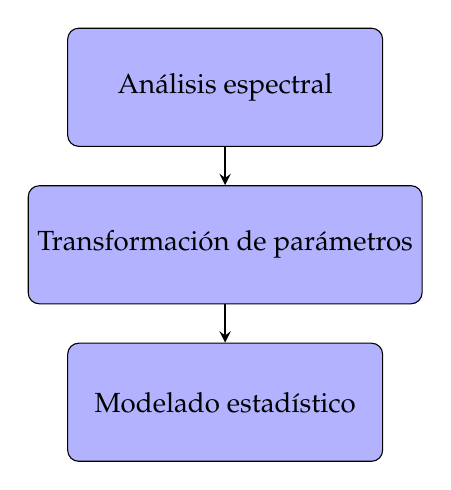
\begin{tikzpicture}[node distance=2cm]
		\node (i1) [startstop] {Análisis espectral};
		\node (i2) [startstop, below of=i1] {Transformación 	de parámetros};
		
		\node (i3) [startstop, below of=i2] {Modelado estadístico};

		\draw [arrow] (i1) -- (i2) ;
		\draw [arrow] (i2) -- (i3);

		\end{tikzpicture}
	\end{center}
	\caption{Etapas de extracción de características \\ Fuente:  \textit{Fuente Propia}}
\end{figure}
\subsection{Algoritmos}
 A continuación describiremos algunos algoritmos que se usan para realizar este proceso.
\subsubsection{Real Cepstral Coefficient(RCC)}
Este algoritmo convierte la señal del dominio de tiempo a dominio de frecuencia aplicando la transformada rápida de fourier a cada cuadro(frame). Luego se aplica le logaritmo y la transforma de fourier inversa. 
\begin{equation}
\label{STs}
\begin{aligned}
Real Cepstrum = IFFT (log (FFT (s (n))))
\end{aligned}
\end{equation}
Donde:
\begin{itemize}
	\item IFFT: Transformada de fourier inversa
	\item FFT: transformada rápida de fourier.
	\item s(n): señal de voz.
\end{itemize}
\subsubsection{Mel Frequency Cepstral Coefficients (MFCC)} 
Es el algoritmo más usado en aplicaciones de reconocimiento de voz, esta basado en el sistema auditivo humano, el cual es sensible a 2 características dinámicas y estáticas. El MFCC se concentra principalmente en las características estáticas. A continuación describiremos el proceso de la MFCC.
\begin{enumerate}
	\item \textbf{Pre-emphasis\\}
	En este paso la señal pasa a través de un filtro el cual enfatiza las altas frecuencia. Este proceso aumentará la potencia de la señal con mayor frecuencia.
	\item \textbf{Framing\\}
	Se realiza la segmentación de la señal de voz digital, es decir la señal es divida en pequeños intervalos(\textit{frames}), estos generalmente son del rango de 20ms a 30ms.

	\item \textbf{Hamming windowing\\}
	Se utiliza como una forma de ventana que trabajo con los bloques de la cadena de extracción de características y tiene la finalidad de integrar las frecuencias más cercanas.
	\begin{equation}
	\label{STs3}
	\begin{aligned}
	Y(n)&= X(n) x W(n)\\
	W(n)&=0.54-0.46\cos(\frac{2\pi n}{N-1})    0\leq n\leq N
	\end{aligned}
	\end{equation}
	\begin{itemize}
		\item $Y(n)$: Señal de salida
		\item $W(n)$: Hamming window
		\item $X(n)$: Señal de entrada
		\item $N$: Número de ejemplo en cada frame
	\end{itemize}
	\item \textbf{Transformada rápida de Fourier\\} 
	Se encarga de transformar las muestras N del dominio de tiempo al dominio de frecuencia.
	\begin{equation}
		\label{TFF}
		\begin{aligned}
		Y(w)= FFT(H(t)\ast X(t))= H(w) \ast X(w)
		\end{aligned}
	\end{equation}
		\begin{itemize}
			\item $Y(w)$: Transformada de Fourier de Y(t)
			\item $H(w)$: Transformada de Fourier de H(t)
			\item $X(w)$: Transformada de Fourier de X(t)

		\end{itemize}
	
	\item \textbf{Mel filter bank\\}
	Debido a que el rango en el espectro de la Transformada rápida de Fourier es muy amplia y la señal de voz no sigue una escala lineal.
	
	La ecuación 4.5 se usa para calcular Mel para una frecuencia de tiempo.
		\begin{equation}
			\label{TFFs}
			\begin{aligned}
			F(mel)=(2595\ast log10(1+f)700)
			\end{aligned}
		\end{equation}	
		
		
		\begin{figure}[H]
			\centering
			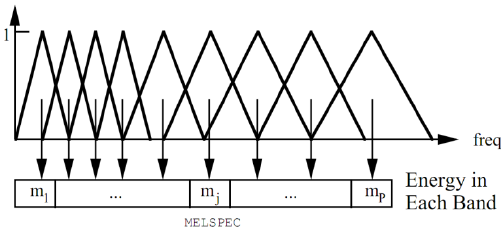
\includegraphics[width=0.7\textwidth]{Figures/melfilter.png}
			\caption{Aplicación del filtro Mel \\ Fuente:  \href{https://www.researchgate.net/figure/Mel-Scale-Filter-Bank-14\_fig2\_280027126}{\textit{https://www.researchgate.net}}}
			\label{onda}
		\end{figure} 
	\item \textbf{Discrete Cosine Transform (DCT)\\}
	Este proceso se encarga de convertir el log del espectro Mel en un dominio de tiempo usando DCT. El resultado es llamado MFCC. El conjunto de coeficientes esa llamado vectores acústicos.
	\item \textbf{Delta energy and Delta spectrum\\}
	La señal de voz junto con los cambios de frames necesitan añadir características relacionadas a los cambios en las características cepstrales sobre el tiempo. La energía en un frame de tiempo $t_{1}$ a $t_{2}$ esta dado por:
	
	\begin{equation}
		\label{energia}
		\begin{aligned}
			Energia=\sum X^{2}(t)
		\end{aligned}
	\end{equation}	
\end{enumerate}
\subsubsection{Codificación lineal predictiva} 
Este método también conocido como LCP considera que la señales de voz pueden ser expresadas como la combinación lineal de las anteriores, entonces podemos describir a la señal de voz utilizando los coeficientes de esta combinación lineal. Este método ha sido utilizado para el procesamiento de la señal de voz debido modela el comportamiento del tracto vocal.\\ En el ecuación 4.3 vemos como se expresa la señal de voz $s$ usando las p anteriores señales de voz y los $a_{k}$ representan \textit{coeficientes del LCP.}

\begin{equation}
\label{LPC}
\begin{aligned}
s(n)= \sum_{k=1}^{p}a_{k}s(n-k)+e(n)
\end{aligned}
\end{equation}



\section{Coincidencia de patrones}
A continuación se describirán algunos algoritmos usados para las tareas de las coincidencias de patrones.

\subsubsection{Modelo oculto de Markov (HMM)}
Es un modelo estadístico donde asumimos que nuestro sistema es un proceso de markov con parámetros desconocidos. A continuación se describirá el proceso en la figura 4.7

\begin{figure}[H]
	\centering
	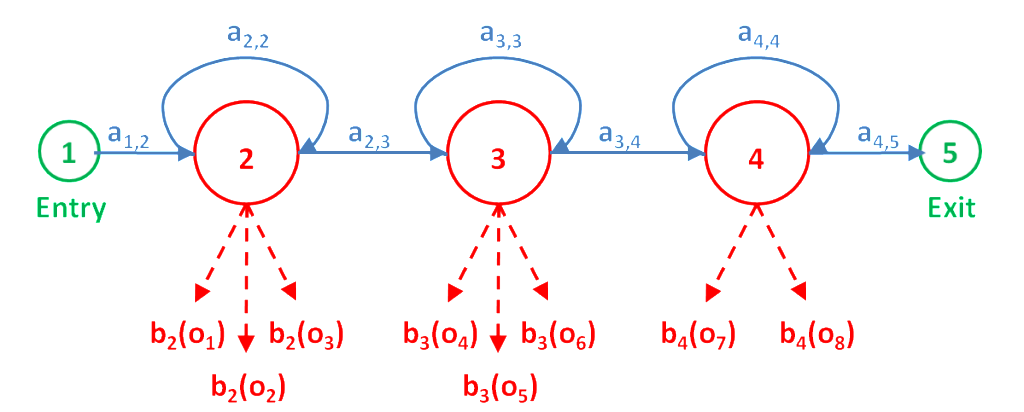
\includegraphics[width=0.6\textwidth]{Figures/hmm}
	\caption{Esquema del HMM\\ Fuente:  \href{http://gekkoquant.com/2014/05/18/hidden-markov-models-model-description-part-1-of-4/}{\textit{http://gekkoquant.com}}}
	\label{}
\end{figure} 
\begin{itemize}
	\item N: Número de estados en el HMM
	\item $a_{ij}$ probabilidad de transición del estado $i$ al $j$.
	\item $	b_{j}(o)$ Probabilidad de generar un vector de característica en estado j.
	
\end{itemize}
\subsubsection{Máquinas de soporte Vectorial(SVM)}
Las SVM usan el concepto de planos de decisión. Un plano de decisión separa un conjunto de objetos que tienes diferentes etiquetas de clases. Las SVM no están restringidas a los problemas lineales debido a las \textit{funciones Kernel.}
\textbf{Funciones Kernels}\\
Las SVM pueden tener distintos tipos de kernels que tienen como objetivo tomar la data y transformarla. Algunas funciones kernels conocidas:
\begin{itemize}
	\item Lineal: $\ker(x_{i},x_{j})= x_{i} \cdot x_{j}$
	\item Polinomial: $\ker(x_{i},x_{j})= ( \gamma x_{i} \cdot x_{j}+C)^d$
	\item Radial: $\ker(x_{i},x_{j})= e^{(\gamma |x_{i} - x_{j}|)}$
	\item Sigmoidal: $\ker(x_{i},x_{j})= \tanh ( \gamma x_{i} \cdot x_{j}+C)$
\end{itemize}
En la figura 4.7 muestra el efecto de las funciones kernels en un conjunto de datos para que este sea linealmente separable sin necesidad de construir curvas complejas.\\
\begin{figure}[H]
	\centering
	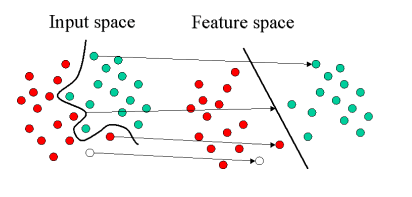
\includegraphics[width=0.9\textwidth]{Figures/svm.png}
	\caption{transformación con la función kernel \\ Fuente:  \href{http://www.statsoft.com/Textbook/Support-Vector-Machines}{\textit{www.statsoft.com}}}
	\label{transformación con la función kernel}
\end{figure} 

\subsubsection{Alineamiento temporal dinámico (DTW)}
Es un método de programación dinámica que busca encontrar una alineación óptima entre 2 series de tiempo. El algoritmo trata de buscar deformaciones entre las series de tiempo y determina la similitudes entre ambas series. Esto nos permite tener una robustez en caso de grupos fonéticos en el audio tenga una duración más prolongada.\\ En la figura 4.6 se muestra 2 series de tiempo donde se trazan las coincidencias entre ambas series.

\begin{figure}[H]
	\centering
	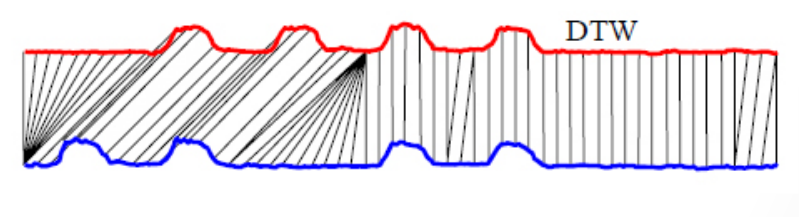
\includegraphics[width=0.9\textwidth]{Figures/dtw.png}
	\caption{DTW\\ Fuente:  \href{https://lemonzi.files.wordpress.com/2013/01/dtw.pdf}{\textit{https://lemonzi.files.wordpress.com}}}
	\label{onda}
\end{figure} 

\subsubsection{Redes Neuronales}
Las redes neuronales descritas en el capítulo 3, luego de su entrenamiento serán capaces de reconocer los patrones de las señales de voz.
%\newpage
$\ $
%\thispagestyle{empty} % para que no se numere esta pagina
\chapter{Implementación}
En este capítulo describiremos detalles de la implementación de nuestro modelo de reconocimiento de números en español. Comenzaremos describiendo el proceso de obtención y tratamiento de datos. Finalmente, mostraremos el esquema de nuestra red neuronal.

\section{Datos}
Para las tareas de reconocimiento de voz es importante encontrar un conjunto de datos adecuado, este servirá para alimentar nuestra red neuronal. Proyectos como \textit{VoxForge}\cite{WEBSITE:21} y \textit{Common Voice}\cite{WEBSITE:22} son iniciativas open source que buscan formar un gran corpus de data para distintos idiomas. Sin embargo en el lenguaje español los datos aún están en proceso de recolección. Por lo cual obtener los datos para una tarea específica resulta complicado.
\subsection{Recolección de datos}
Debido al problema anterior fue necesario realizar una propia recolección de datos. Durante este proceso se obtuvo la información de 12 hablantes. Los cuales proporcionaron grabaciones de voz de la pronunciación de los dígitos $0, 1, .. ., 8, 9$. 
\subsubsection{Conjuntos de datos}
Nuestro conjunto de datos consta de un total de 300 audios los cuales fueron dividos en 2 conjuntos:
\begin{itemize}
	\item \textbf{Training}: Este conjunto es usado para entrenar nuestro modelo. Posee 24 muestra de cada número.
	\item \textbf{Test}: Este conjunto es usar para verificar la precisión de modelo. Posee 11 muestras de cada número.
\end{itemize}

La división del conjunto de datos es mostrada en el cuadro 5.1.

\begin{table}[H]
	\centering
	\begin{tabular}{|c|c|}
		\hline
		\rowcolor{Gray}	Training & Test \\ \hline
		240      & 110   \\ \hline
	\end{tabular}
	\caption{División del conjunto de datos}
\end{table}
Debido a las diferencias de entre las voces de entre personas de diferentes sexos fue necesario tener una variedad de hablantes entre mujeres y varones con el objetivo de construir un modelo más robusto. La distribución de hablantes se muestra en cuadro 5.2.


\begin{table}[H]
	\centering
	\begin{tabular}{|c|c|}
		\hline
		\rowcolor{Gray}Mujeres & Varones \\ \hline
		5      & 7   \\ \hline
	\end{tabular}
	\caption{Distribución de hablantes del conjunto de datos por sexo}
\end{table}


La distribución de acuerdo a la cantidad de audios con Voces Femeninas(VF) y Voces Masculinas(VM) se muestran en el cuadro 5.3.

\begin{table}[H]
	\centering
	\begin{tabular}{|c|c|c|c|}
		\hline
		\rowcolor{Gray} 	\multicolumn{4}{|c|}{conjunto de datos}                    \\ \hline
		\multicolumn{2}{|c|}{Training} & \multicolumn{2}{c|}{Test} \\ \hline
		VF              & VM             & VF          & VM           \\ \hline
		90             & 150           & 40          & 70         \\ \hline
	\end{tabular}
	\caption{División del conjunto en base a la cantidad de audios con voces femeninas y masculinas}
\end{table}

\subsection{Tratamiento de los datos}

\subsubsection{Conversión de formato}
Los audios proporcionados por algunos hablantes se encontraban en un formato ogg, el cual tuvo que ser transformado al formato wav para su procesamiento esto debido a que ogg es más formato usado en teléfonos moviles mientras que el formato wav es más estándar.
\begin{lstlisting}[language=Bash,caption=Bash para conversión de formato,captionpos=b]
# itera los archivos .ogg
for i in *.ogg;
# realiza la conversion ogg a wav usando ffmpeg
do ffmpeg -i "$i" "${i%.*}.wav"; 
done

\end{lstlisting}
\subsection{Obtención de coeficientes cepstrales}
Nuestro modelo será alimentado con audios pero antes se necesita obtener la información más importante y eliminar el ruido de fondo. Para esto utilizamos el algoritmo de extracción de características MFCC  (Ver Cap4.).\\  Para estas tareas hacemos uso de las librerías: \textit{librosa, sklearn y numpy}.\\\ Estas son usadas en el código 5.2. donde se obtiene 20 coeficientes cepstrales de una muestra.
\begin{lstlisting}[language=Python,caption=Obtención de MFCC,captionpos=b]
# cargado del audio
wave, sr = librosa.load(DIR+dir, mono=True)
# obtencion de los coeficientes
features= librosa.feature.mfcc(wave, sr,n_mfcc=20)
#padding con ceros asegurar misma dimension de salida
features=np.pad(features,((0,0),(0,160-len(features[0]))),
mode='constant',constant_values=0)

\end{lstlisting}

\subsection{One Hot encoding }
Para entrenar nuestro modelo necesitamos representar nuestras clases o variables categóricas de manera numérica la cual es más útil para tareas de clasificación y regresión. Una forma de lograr esto es mediante el uso de One Hot enconding. En la figura 5.1 podemos representar las clases red, green y blue, en vectores únicos de dimensión 3.

\begin{figure}[H]
	\centering
	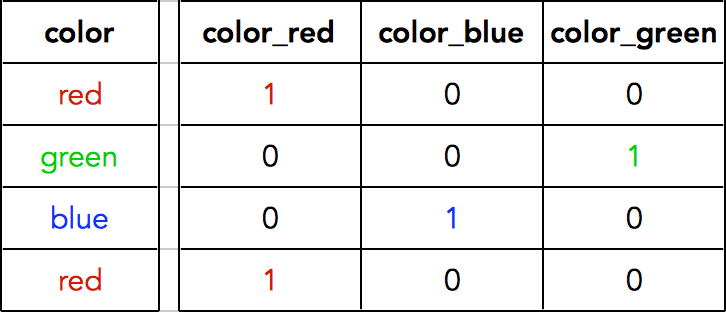
\includegraphics[width=0.6\textwidth]{Figures/one_hot_encoding}
	\caption{Ejemplo One hot encoding \\ Fuente:  \href{https://www.machinelearningplus.com/machine-learning/caret-package/attachment/one-hot-encoding/}{\textit{https://www.machinelearningplus.com/}}}
	\label{one}
\end{figure} 
En nuestra implementación fue necesario encontrar una representación para nuestras 10 clases de números. A continuación mostramos el código que nos permitió hallar esa representación.
\begin{lstlisting}[language=Python,caption=one hot encoding,captionpos=b,xleftmargin=.05\textwidth]
# importacion de libreria
from sklearn.preprocessing import OneHotEncoder
# vocabulario de clases definidas
vocabulary_words=np.array(['cero','uno','dos','tres',
'cuatro','cinco','seis','siete','ocho','nueve'])
# creacion del objeto OneHotEncoder
onehot_encoder = OneHotEncoder(handle_unknown='ignore',
categories='auto')
# entrenamiento del OneHotEncoder en base a las clases definidas
onehot_encoder.fit(X=vocabulary_words.reshape(-1,1))
\end{lstlisting}

\section{Modelo de la red neuronal}

En esta sección  veremos algunos modelos que fueron entrenados para la tarea de clasificación de audios de números estos serán probados con un solo tipo de redes RNN y en especial su derivado LSTM.
\subsection{RNN}
Definimos un red neuronal con una sola capa RNN y una capa densamente conectada.

\begin{lstlisting}[language=Python,caption=Modelo LSTM,captionpos=b,xleftmargin=.05\textwidth]
# establece la secuencia para empezar con el apilado de capas
model=tf.keras.Sequential()
# se apila una capa RNN simple 
model.add(tf.keras.layers.SimpleRNN(128, input_shape=(time_steps,n_inputs)))
# establece una capa densamente conectada
model.add(tf.layers.Dense(n_class, activation='softmax'))

\end{lstlisting}


\subsection{LSTM}
Para LSTM veremos modelo sin la aplicación de la capa Dropout y modelos con esta capa.


Nuestro modelo fue definido usando keras como muestra el código 5.3 

\begin{center}
\begin{lstlisting}[language=Python,caption=Modelo LSTM,captionpos=b,xleftmargin=.05\textwidth]
# usado para apilar las capas de la red
model=tf.keras.Sequential()
# apila una capa LSTM
model.add(tf.keras.layers.LSTM(n_units,
 input_shape=(time_steps,n_inputs)))
# apila un Dropout a nuestra red para evitar overfitting
model.add(tf.keras.layers.Dropout(0.5))
# establece una capa densamente conectada
model.add(tf.layers.Dense(n_class, activation='softmax'))


\end{lstlisting}
\end{center}



Para entrenamiento de nuestro modelos usaremos los parámetros mostrados en el código 5.4, categorical crossentropy será nuestra función de perdida y nuestro optimizador será Adam.s

\begin{lstlisting}[language=Python,caption=Parámetros para el entrenamiento del modelo,captionpos=b,xleftmargin=.05\textwidth]
# configura el entrenamiento del modelo
model.compile(loss='categorical_crossentropy',
optimizer='adam',metrics=['accuracy'])
\end{lstlisting}
\chapter{Conclusiones y Trabajo Futuro}
En este capítulo se describirán las conclusiones generales que se encontraron al probar y estudiar los distintos métodos de optimización utilizados para el proceso de acelerar el entrenamiento de nuestra 2 redes neuronales convolucionales en los dataset CIFAR-10 y CIFAR-100.\\ Además, se propondrán algunas mejoras para que el trabajo obtenga mejores resultados.


\section{Conclusiones}


\begin{itemize}

\item[•] Los métodos de optimización Adam y RMSprop obtuvieron los mejores resultados de precisión en ambas pruebas.

\item[•] A pesar de que el método de optimización Adam fue propuesto a partir del RMSprop. Adam fue superado en algunas de pruebas realizadas.
\item[•] Entre los métodos adaptativos Adam, RMSprop y Adagrad . Solo este último obtuvo los peores resultados, esto se debió a su dificultad de trabajar con la suma de las gradientes al cuadrado lo cual poco a poco redujo su tasa de aprendizaje.
\item[•] El RMSprop como una mejora del Adagrad, obtuvó mejores resultados que este último. Esto debido a que RMSprop trabaja con el promedio de la raíz de la gradiente anterior y tasas de decaimiento para controlar el problema de la disminución de la tasa de aprendizaje del método Adagrad.
\item[•] Adam es el método que tiene un decaimiento más acelerado al calcular el error en la función de costo cross-entropy.

\end{itemize}


\section{Trabajo Futuro}
El propósito general de este seminario I fue adquirir el conocimiento y experiencia necesarios para poder trabajar con redes neuronales profundas. Los métodos de optimización fueron una manera de introducirme al área de las redes convolucionales y comprender las ventajas y desventajas de algunos métodos. \\
Los temas de aprendizaje automático y en particular del aprendizaje profundo son muy amplios y en este seminario se trato de acoplar los temas pero no se realizó un análisis más detallado debido a la amplitud del área. \\
En el Seminario II se trabajará con más detalle el campo de redes neuronales convolucionales, además se tratará de diseñar un red neuronal convolucional y comparar este modelo con algunos actualmente usados. Además de realizar un implementación más interactiva .\\ Este seminario fue limitado debido a la capacidad de la tarjeta gráfica usada ya que en algunos ensayos la memoria era insuficiente para el futuro seminario se planea realizar las pruebas en mejores equipos como por ejemplo contratar servicios de máquinas virtuales de Amazon u otro proveedor.



%\afterpage{\blankpage}\textsl{}
\bibliography{main}
\bibliographystyle{unsrt}
\afterpage{\blankpage}
\appendix
% Appendix A

\chapter{Arquitectura de la red y Resultados obtenidos} % Main appendix title

\label{AppendA} % For referencing this appendix elsewhere, use \ref{AppendixA}
\section{Capas de la red neuronal convolucional}

\begin{figure}[H]
		\begin{center}
		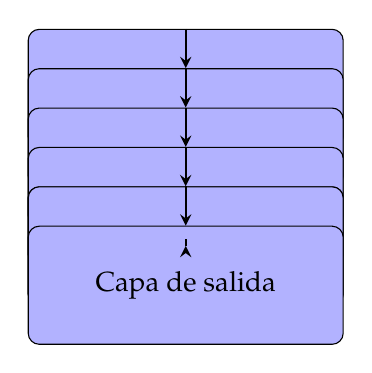
\begin{tikzpicture}[node distance=0.5cm]
		\node (input) [startstop] {Capa de Entrada};
		\node (conv1) [startstop, below of=input] {Capa de convolución 1};
		
		\node (pool1) [startstop, below of=conv1] {Capa Pooling 1};
		\node (conv2) [startstop, below of=pool1] {Capa de convolución 2};
		\node (pool2) [startstop, below of=conv2] {Capa Pooling 2};
		\node (full) [startstop, below of=conv2] {Full Layer};
		\node (exit) [startstop, below of=full] {Capa de salida};
		\draw [arrow] (input) -- (conv1) ;
		\draw [arrow] (conv1) -- (pool1);
		\draw [arrow] (pool1) -- (conv2);
		\draw [arrow] (conv2) -- (pool2);
		\draw [arrow] (pool2) -- (full);
		\draw [arrow] (full) -- (exit);
		\end{tikzpicture}
	\end{center}
	\caption{Capas de la red neuronal usada \\ Fuente:  \textit{Fuente Propia}}
\end{figure}



\section{Resultados de precisión de entrenamiento}
\subsection{CIFAR-10}
\begin{figure}[H]
	\begin{centering}
		\subfloat[fig 1]{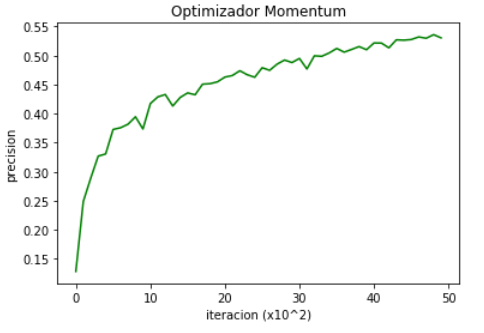
\includegraphics[width=0.45\textwidth]{Figures/momemtum5000.png}} 
		\subfloat[fig 2]{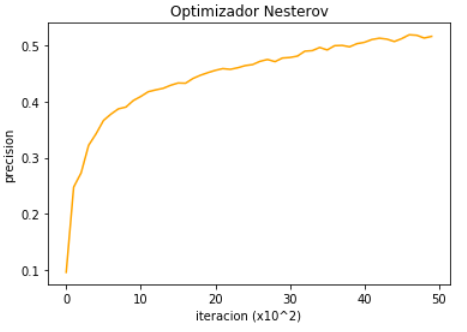
\includegraphics[width=0.45\textwidth]{Figures/nesterov5000.png}}\\
		\subfloat[fig 3]{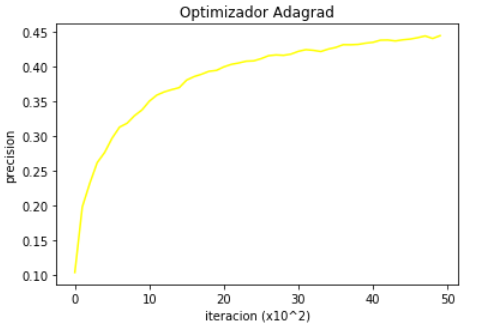
\includegraphics[width=0.45\textwidth]{Figures/adagrad5000.png}}
		\subfloat[fig 3]{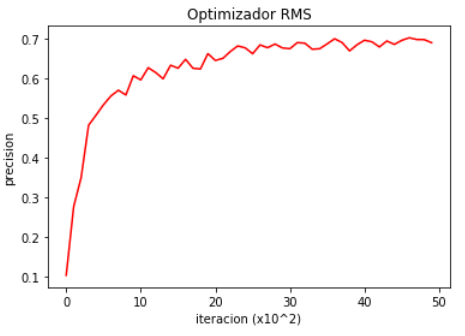
\includegraphics[width=0.45\textwidth]{Figures/rms5000.png}}\\
		\subfloat[fig 4]{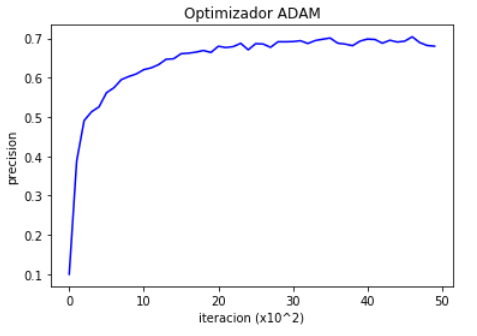
\includegraphics[width=0.5\textwidth]{Figures/adam5000.png}} 
		\caption{optmizadores 5000 epochs \\ Fuente :{\textit{Fuente Propia}}}
		\label{some example0}
	\end{centering}

\end{figure}


\begin{figure}[H]
	\begin{centering}
		\subfloat[fig 1]{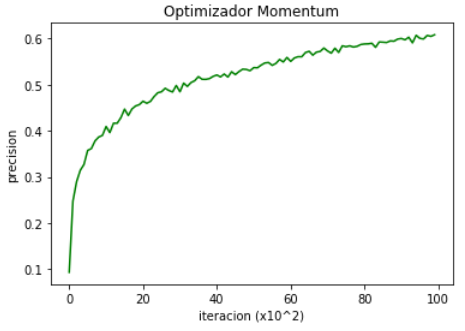
\includegraphics[width=0.55\textwidth]{Figures/momemtum10000.png}} 
		\subfloat[fig 2]{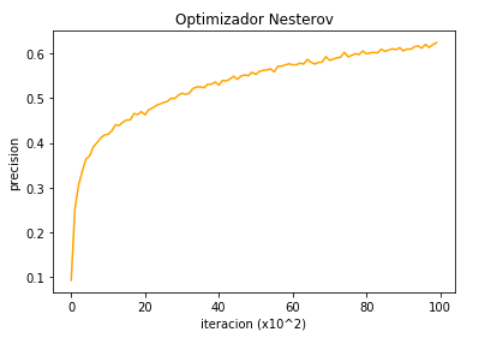
\includegraphics[width=0.55\textwidth]{Figures/nesterov10000.png}}\\
		\subfloat[fig 3]{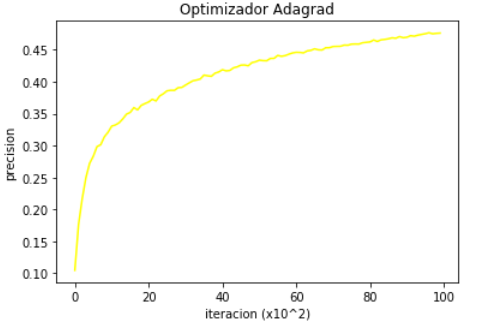
\includegraphics[width=0.55\textwidth]{Figures/adagrad10000.png}}
		\subfloat[fig 3]{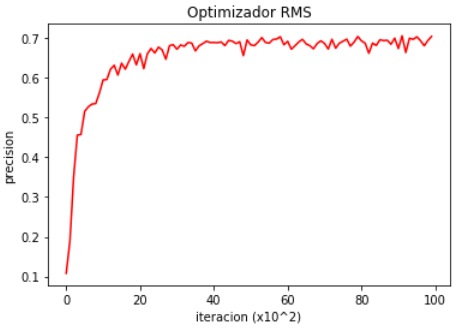
\includegraphics[width=0.55\textwidth]{Figures/rms10000.png}}\\
		\subfloat[fig 4]{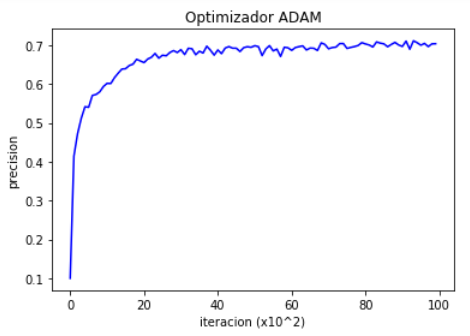
\includegraphics[width=0.6\textwidth]{Figures/adam10000.png}} 
		\caption{optmizadores 10000 epochs\\ Fuente:  \textit{Fuente Propia}}
		\label{some example1}
	\end{centering}
	
\end{figure}

\begin{figure}[H]
	\begin{centering}
		\subfloat[fig 1]{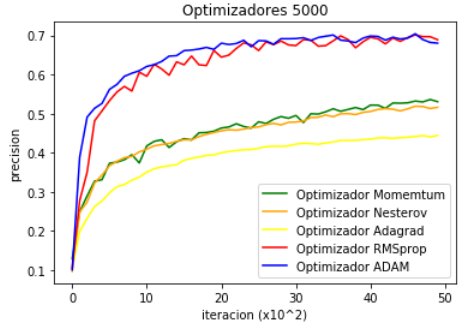
\includegraphics[width=0.8\textwidth]{Figures/optimizadores5000.png}} 
		\caption{Comparación de precisión de optimizadores para 5000 epochs\\ Fuente:  \textit{Fuente Propia}}
		\label{some example2}
	\end{centering}
	
\end{figure}

\begin{figure}[H]
	\begin{centering}
		\subfloat[fig 1]{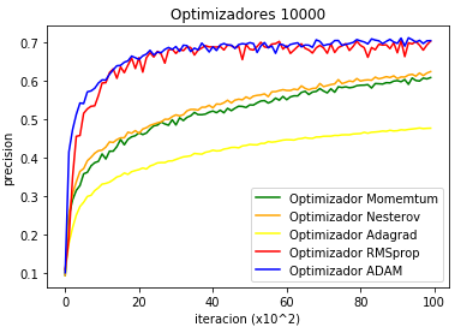
\includegraphics[width=0.8\textwidth]{Figures/optimizadores10000.png}} 
		\caption{Comparación de optimizadores para 10000 epochs\\ Fuente:  \textit{Fuente Propia}}
		\label{some example3}
	\end{centering}
	
\end{figure}

\subsection{CIFAR-100}

\begin{figure}[H]
	\begin{centering}
		\subfloat[fig 1]{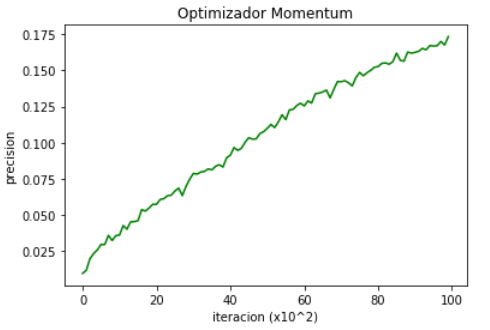
\includegraphics[width=0.55\textwidth]{Figures/100momemtum10000.png}} 
		\subfloat[fig 2]{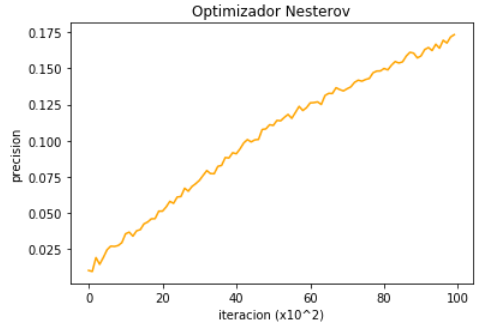
\includegraphics[width=0.55\textwidth]{Figures/100nesterov10000.png}}\\
		\subfloat[fig 3]{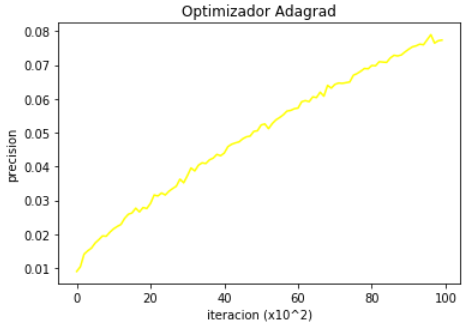
\includegraphics[width=0.55\textwidth]{Figures/100adagrad10000.png}}
		\subfloat[fig 3]{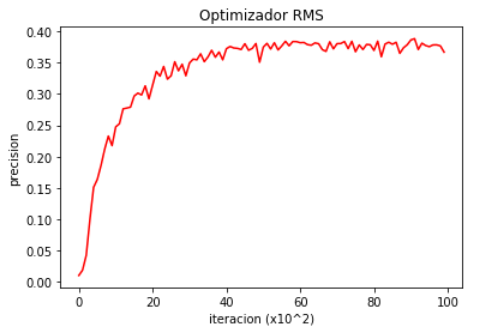
\includegraphics[width=0.55\textwidth]{Figures/100rms10000.png}}\\
		\subfloat[fig 4]{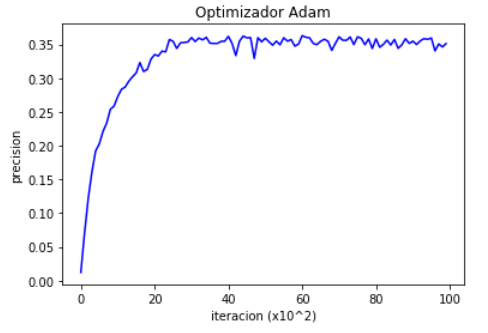
\includegraphics[width=0.6\textwidth]{Figures/100adam10000.png}} 
		\caption{optmizadores 10000 epochs\\ Fuente:  \textit{Fuente Propia}}
		\label{some exampleasa1}
	\end{centering}
	
\end{figure}



\begin{figure}[H]
	\begin{centering}
		\subfloat[fig 1]{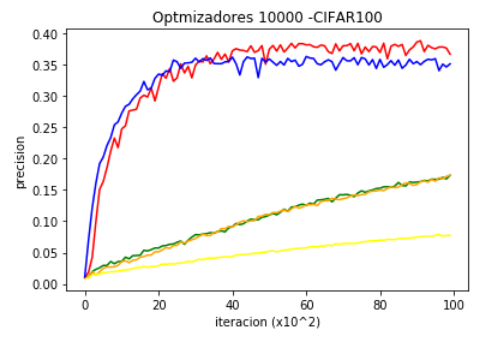
\includegraphics[width=0.8\textwidth]{Figures/cifar100result.png}} 
		\caption{Comparación de optimizadores para 10000 epochs - CIFAR100\\ Fuente:  \textit{Fuente Propia}}
		\label{some example32}
	\end{centering}
	
\end{figure}
\section{Resultados del error en el entrenamiento}
\subsection{CIFAR-10}
\begin{figure}[H]
	\begin{centering}
		\subfloat[fig 1]{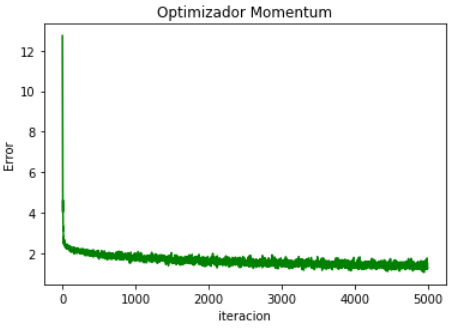
\includegraphics[width=0.5\textwidth]{Figures/momemtumcross5000.png}} 
		\subfloat[fig 2]{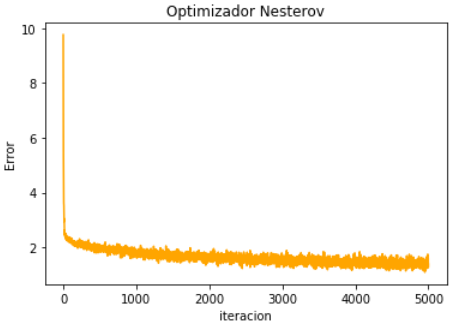
\includegraphics[width=0.5\textwidth]{Figures/nesterovcross5000.png}}\\
		\subfloat[fig 3]{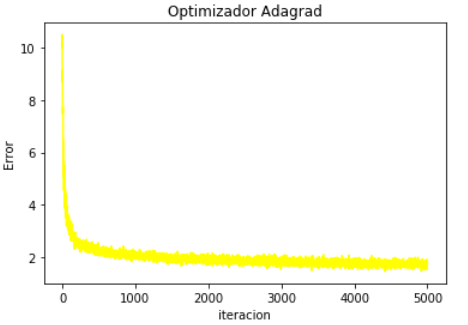
\includegraphics[width=0.5\textwidth]{Figures/adagradcross5000.png}}
		\subfloat[fig 3]{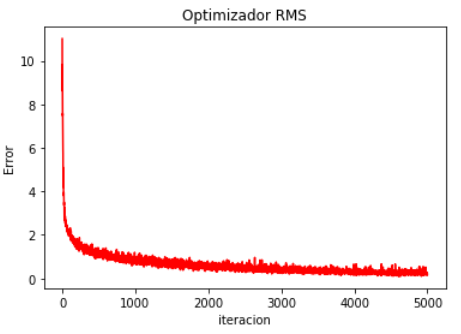
\includegraphics[width=0.5\textwidth]{Figures/rmscross5000.png}}\\
		\subfloat[fig 4]{\includegraphics[width=0.5\textwidth]{Figures/adamcross5000.png}} 
		\caption{Error en los optimizadores 5000 epochs\\ Fuente:  \textit{Fuente Propia}}
		\label{some}
	\end{centering}
	
\end{figure}

\begin{figure}[H]
	\begin{centering}
		\subfloat[fig 1]{\includegraphics[width=0.8\textwidth]{Figures/optimizadorescross5000050}} 
		\caption{Comparación de las funciones de costo rango 0-50\\ Fuente:  \textit{Fuente Propia}}
		\label{some example5}
	\end{centering}
	
\end{figure}

\begin{figure}[H]
	\begin{centering}
		\subfloat[fig 1]{\includegraphics[width=0.8\textwidth]{Figures/optimizadorescross50000500}} 
		\caption{Comparación de las errores rango 0-500\\ Fuente:  \textit{Fuente Propia}}
		\label{some example6}
	\end{centering}
	
\end{figure}
\begin{figure}[H]
	\begin{centering}
		\subfloat[fig 1]{\includegraphics[width=0.6\textwidth]{Figures/momemtumcross10000.png}} 
		\subfloat[fig 2]{\includegraphics[width=0.6\textwidth]{Figures/nesterovcross10000.png}}\\
		\subfloat[fig 3]{\includegraphics[width=0.6\textwidth]{Figures/adagradcross10000.png}}
		\subfloat[fig 3]{\includegraphics[width=0.6\textwidth]{Figures/RMScross10000.png}}\\
		\subfloat[fig 4]{\includegraphics[width=0.6\textwidth]{Figures/adamcross10000.png}} 
		\caption{Error en los optimizadores 10000 epochs -CIFAR10\\ Fuente:  \textit{Fuente Propia}}

	\end{centering}
	
\end{figure}

\subsection{CIFAR-100}
\begin{figure}[H]
	\begin{centering}
		\subfloat[fig 1]{\includegraphics[width=0.6\textwidth]{Figures/100momentumcross10000.png}} 
		\subfloat[fig 2]{\includegraphics[width=0.6\textwidth]{Figures/100nesterovcross10000.png}}\\
		\subfloat[fig 3]{\includegraphics[width=0.6\textwidth]{Figures/100adagradcross10000.png}}
		\subfloat[fig 3]{\includegraphics[width=0.6\textwidth]{Figures/100rmscross10000.png}}\\
		\subfloat[fig 4]{\includegraphics[width=0.6\textwidth]{Figures/100adamcross10000.png}} 
		\caption{Error en los optimizadores con 10000 epochs - CIFAR 100 \\ Fuente:  \textit{Fuente Propia}}
		\label{some2341}
	\end{centering}
	
\end{figure}

\begin{figure}[H]
	\begin{centering}
		\subfloat[fig 1]{\includegraphics[width=0.8\textwidth]{Figures/cifar100error.png}} 
		\caption{Comparación los errores rango 9900-10000\\ Fuente:  \textit{Fuente Propia}}
		\label{COMPARACION}
	\end{centering}
	
\end{figure}


\end{document}